\documentclass[10pt,portrait, twocolumn]{article}
\usepackage{multicol}
\usepackage{calc}
\usepackage[portrait]{geometry}
\usepackage{amsmath,amsthm,amsfonts,amssymb}
\usepackage{times}
\usepackage{color,graphicx,overpic}
\graphicspath{ {images/} }
\usepackage{hyperref}
\usepackage{pgfplots}
\usepackage{esint}
\usepackage{bm}
\usepackage{tikz}
\usepackage{relsize}
\usepackage{datetime}
\usepackage[utf8] {inputenc}
\usepackage[spanish, activeacute] {babel}
\usepackage{IEEEtrantools}
\usepackage{framed}

\usepackage{pdflscape}


%\usepackage{draftwatermark}
%\SetWatermarkText{Javier de Martín}
%\SetWatermarkScale{0.8}

% This sets page margins to .5 inch if using letter paper, and to 1cm
% if using A4 paper. (This probably isn't strictly necessary.)
% If using another size paper, use default 1cm margins.
\geometry{top=.5cm,left=.5cm,right=.5cm,bottom=.5cm}
    
\pgfplotsset{
    dirac/.style={
        mark=triangle*,
        mark options={scale=2},
        ycomb,
        scatter,
        visualization depends on={y/abs(y)-1 \as \sign},
        scatter/@pre marker code/.code={\scope[rotate=90*\sign,yshift=-2pt]}
    }
}

% Turn off header and footer
\pagestyle{empty}

% Redefine section commands to use less space
\makeatletter
\renewcommand{\section}{\@startsection{section}{1}{0mm}%
                                {-1ex plus -.5ex minus -.2ex}%
                                {0.5ex plus .2ex}%x
                                {\normalfont\large\bfseries}}
\renewcommand{\subsection}{\@startsection{subsection}{2}{0mm}%
                                {-1explus -.5ex minus -.2ex}%
                                {0.5ex plus .2ex}%
                                {\normalfont\normalsize\bfseries}}
\renewcommand{\subsubsection}{\@startsection{subsubsection}{3}{0mm}%
                                {-1ex plus -.5ex minus -.2ex}%
                                {1ex plus .2ex}%
                                {\normalfont\small\bfseries}}
\makeatother

\newcommand{\Lagr}{\mathcal{L}}

% Define BibTeX command
\def\BibTeX{{\rm B\kern-.05em{\sc i\kern-.025em b}\kern-.08em
    T\kern-.1667em\lower.7ex\hbox{E}\kern-.125emX}}

% Don't print section numbers
\setcounter{secnumdepth}{0}


\setlength{\parindent}{0pt}
\setlength{\parskip}{0pt plus 0.5ex}

%My Environments
\newtheorem{example}[section]{Example}
% ---------------------------------------------------------------

\begin{document}

\begin{landscape}

\raggedright
\footnotesize
\begin{multicols}{2}


% multicol parameters
% These lengths are set only within the two main columns
%\setlength{\columnseprule}{0.25pt}
\setlength{\premulticols}{1pt}
\setlength{\postmulticols}{1pt}
\setlength{\multicolsep}{1pt}
\setlength{\columnsep}{2pt}

\begin{framed}
	\begin{center}
    	\Large{\underline{Sistemas de Telecomunicación}} \\
    	\scriptsize{3º Ingeniería de Telecomunicaciones | UPV/EHU}\\
     	%Actualizado por última vez el \today \\
     	"\textsl{Under-promise and over-deliver}." \\
     	%\hspace{5 pt} \\
     	\small{\textbf{Javier de Martín -- 2016}}
	\end{center}
\end{framed}

%
% Cheatsheet code below 
%                                                      

\section{\underline{Unidades Logarítmicas}}

%\begin{center}
%	\begin{tikzpicture}
%		\node [draw, align=center] (1) at (0,0) {Fuente};
%		\node [draw, align=center] (2) at (0,-1) {Procesado en TX};
%	
%		\node [draw, align=center] (3) at (2,-1) {Red};
%		
%		\node [draw, align=center] (4) at (4,-1) {Procesado en RX};
%		\node [draw, align=center] (5) at (4,0) {Presentación};
%	
%		\path (1) edge node [right] {} (2);
%		\path (2) edge node [above] {} (3);
%		\path (3) edge node [above] {} (4);
%		\path (4) edge node [left] {} (5);
%	\end{tikzpicture}	
%\end{center}

\textbf{dB} es una unidad que describe una \textbf{relación} entre magnitudes.

\begin{IEEEeqnarray*}{rCl}
	L(dB) & = & 10 \cdot \log_{10} \left( \frac{P_2}{P_1} \right) \\ & = & 20 \cdot \log_{10} \left( \frac{V_2}{V_1} \right) + 10 \cdot \log_{10} \left( \frac{R_1	}{R_2} \right)
\end{IEEEeqnarray*}

\subsection{Unidades Derivadas del dB}

\begin{itemize}
	\item $dBm$: Potencia de la señal en un punto cualquiera de un circuito referida a una potencia de $1mW$.
		
		\begin{equation*}
			L(dBm) = 10 \cdot \log_{10} \left( \frac{P(mW)}{1mW} \right)
		\end{equation*}
	\item $dBW$: Potencia de la señal referida a una potencia de $1W$.
		
		\begin{equation*}
			L(dBW) = 10 \cdot \log_{10} \left( \frac{P(W)}{1W} \right)
		\end{equation*}
		
	\item $dBmV$: Nivel de un voltaje comparado con $1mV$ sobre una carga de $75\Omega$.
		
		\begin{equation*}
			L(dbmV) = 20 \cdot \log_{10} \left( \frac{V(mV)}{1mV} \right)
		\end{equation*}
		
	\item $dBV$: Nivel de un voltaje comparado con $0.0775 V$ (tensión eficaz) sobre una carga de $600\Omega$.
		
		\begin{equation*}
			L(dBm) = dBV + 10 \cdot \log_{10} \left( \frac{600}{R} \right)
		\end{equation*}
\end{itemize}

Estas medidas están relacionadas por:

	\begin{equation*}
		L(dBm) = L(dBV) + 10 \cdot \log_{10} \left( \frac{600}{R} \right)
	\end{equation*}

\subsection{Niveles}

\begin{itemize}
	\item $dBr$: Expresa el nivel relativo en un punto con respecto a otro punto; es una medida en $dB$ sin sufijo, $r$ se incluye para denotar que se trata de un valor relativo a un cierto punto de referencia.
	
		\begin{equation*}
			L(dBr) = 10 \log_{10} \frac{P}{P_{ref}}
		\end{equation*}
	
	\item $dBm0$: Indica la potencia en $dBm$ presente en el punto de nivel relativo cero.
		
		\begin{equation*}
			L(dBm0) = L_A(dBm) - L_A(dBr)
		\end{equation*}
\end{itemize}

Si se emite un tono de prueba ($0dBm$) $\rightarrow L_A (dBm) = L_A (dBr)$.

\section{\underline{Perturbaciones y Medios de TX}}

\subsection{Distorsión Lineal}

%\begin{center}
%	\begin{tikzpicture}
%		\draw (0,0) -- node[above left] {$x(t)$} (0.6,0);
%		\node [draw, align=center] at (0.95,0) {$h(t)$};	
%		\draw (1.3,0) -- node[above right] {$y(t) = k \cdot x(t - t_0)$} (1.9,0);
%	\end{tikzpicture}	
%\end{center}

%Hay distorsión no lineal si en la banda de trabajo:

\begin{itemize}
	\item de amplitud: $k \neq cte$, $k = k(f)$
	\item de fase: $t_o \neq cte$, $t_0 = t_o(f)$
\end{itemize}

\subsection{Distorsión No Lineal o Armónica}

%No se puede utilizar la respuesta en frecuencia $H(f)$, se utilizará la \textbf{característica de transferencia}.

\begin{IEEEeqnarray*}{rCl}
	y(t) = f(x(t)) \underbrace{=}_\textrm{\tiny{Serie de Taylor}}  \overbrace{a_0}^\textrm{C.C} & + & \overbrace{a_1 x(t)}^\textrm{\tiny{Término Lineal}} + \overbrace{a_2 x^2(t)}^\textrm{\tiny{Término Cuadrático}} + \\ & + & \overbrace{a_3 x^3(t)}^\textrm{\tiny{Término Cúbico}} + ... + a_n x^n(t)
\end{IEEEeqnarray*}

%\begin{center}
%	\begin{tikzpicture}[scale = 0.5]
%	\begin{axis}[axis lines = middle,xmin=-0.1,xmax = 3.2,ymin=-0.3,ymax=3, xticklabels={,,}, yticklabels={,,}] %,grid=both]
%		\addplot +[dirac] coordinates {(1, 2)};
%		
%		% Valores del eje X
%		\node at (axis cs:1, 0) [anchor=north] {$f_0$};
%		\node at (axis cs:0, 3) [anchor=north west] {$X(f)$};
%		\node at (axis cs:3.2, 0) [anchor=south east] {$f$};
%		
%	\end{axis}
%\end{tikzpicture}
%\hspace{2pt}
%$\rightarrow$
%\begin{tikzpicture}[scale = 0.5]
%	\begin{axis}[axis lines = middle,xmin=-0.1,xmax = 3.2, ymin=-0.3,ymax=3, xticklabels={,,}, yticklabels={,,}] %,grid=both]
%		\addplot +[dirac] coordinates {(1, 2)};
%		%\node at (axis cs:1,2) [anchor=north east] {test};
%		\addplot +[orange, dirac] coordinates {(2, 1.6)};
%		\node at (axis cs:2, 1.6) [anchor=north east] {$V_{d_3}$};
%		\addplot +[orange, dirac] coordinates {(3, 1.3)};
%		\node at (axis cs:3, 1.3) [anchor=north east] {$V_{d_3}$};
%		
%		% Valores del eje X
%		\node at (axis cs:1, 0) [anchor=north] {$f_0$};
%		\node at (axis cs:2, 0) [anchor=north] {$ 2 \cdot f_0$};
%		\node at (axis cs:3, 0) [anchor=north] {$3 \cdot f_0$};
%		\node at (axis cs:0, 3) [anchor=north west] {$Y(f)$};
%		\node at (axis cs:3.2, 0) [anchor=south east] {$f$};
%		
%		% Nota: "Amplitud de distorsión
%		\draw [<-] (axis cs:2,1.7)-- +(20pt,15pt) node[above] {Amplitud de distorsión};
%		\draw [<-] (axis cs:3,1.4)-- +(-20pt,30pt) node[above] {}; %{Amplitud de distorsión};
%	\end{axis}
%\end{tikzpicture}
%\end{center}

El grado del polinomio a la salida del sistema no lineal indica cuántas frecuencias nuevas van a ser generadas por dicho sistema.

\begin{itemize}
	\item \textbf{Coeficiente de Distorsión del Armónico n-ésimo $d_n$}:
		\begin{IEEEeqnarray*}{rCl}
			d_n & = & \frac{V_{d_n}}{V_1} \hspace{5pt} n = 2, 3, ..., k \\
			D_n & = & 20 \cdot \log_{10} \frac{V_{d_n}}{V_1}	
		\end{IEEEeqnarray*}
	\item \textbf{Atenuación del Armónico n-ésimo $A_n$}:
		\begin{equation*}
			A_n = 20 \cdot \log_10 \frac{V_1}{V_{d_n}} = -D_n
		\end{equation*}
	\item \textbf{Coeficiente de Distorsión Total $d$}:
		\begin{equation*}
			d = \sqrt{\sum_{n>1} d_n^2}
		\end{equation*}
	\item \textbf{Total Harmonic Distortion(THD)}:
		\begin{equation*}
			THD(\%) = \frac{1}{V_1} \sqrt{\sum_{n>1} V_{d_n}^2} \cdot 100 \%
		\end{equation*}
\end{itemize}

Si $V_1$ aumenta $\Delta (dB) \rightarrow V_{d_n}$ aumenta $n \cdot \Delta (dB)$. 


\subsection{Intermodulación}

\begin{center}
	\begin{tikzpicture}
		\draw (0,0) -- node[above left] {$x(t)$} (0.6,0);
		\node [draw, align=center] at (0.95,0) {$h(t)$};	
		\draw (1.3,0) -- node[above right] {$y(t) = a_0 + a_1 \cdot x(t)+ ... + a_n \cdot x^n(t)$} (1.9,0);
	\end{tikzpicture}	
\end{center}

A la salida del sistema aparecen nuevas frecuencias:

\begin{itemize}
	\item Armónicos: $2 \cdot f_1$, $2 \cdot f_2$, $3 \cdot f_1$, $3 \cdot f_2$, ..., $n \cdot f_1$, $n \cdot f_2$
	\item Combinación lineal de las frecuencias de x(t):
		\begin{itemize}
			\item Segundo orden: $f_1 + f_2$, $f_1 - f_2$, ...
			\item Tercer orden: $2 f_1 + f_2$, $f_1 - 2 f_2$, ... 
		\end{itemize} 
\end{itemize}

\begin{center}
	\begin{tikzpicture}[scale = 0.5]
	\begin{axis}[axis lines = middle,xmin=-0.1,xmax = 3.2,ymin=-0.3,ymax=3, xticklabels={,,}, yticklabels={,,}] %,grid=both]
		\addplot +[dirac, blue] coordinates {(1, 2)};
			\node at (axis cs:1, 2) [anchor=north east] {$V_1$};
		\addplot +[dirac, blue] coordinates {(1.5, 2)};
			\node at (axis cs:1.5, 2) [anchor=north east] {$V_2$};
		
		% Valores del eje X
		\node at (axis cs:1, 0) [anchor=north] {$f_1$};
		\node at (axis cs:1.5, 0) [anchor=north] {$f_2$};
		
		\node at (axis cs:0, 3) [anchor=north west] {$x(t)$};
		\node at (axis cs:3.2, 0) [anchor=south east] {$f$};
		
	\end{axis}
\end{tikzpicture}
\hspace{2pt}
$\rightarrow$
\begin{tikzpicture}[scale = 0.5]
	\begin{axis}[axis lines = middle,xmin=-0.1,xmax = 5, ymin=-0.4,ymax=3, xticklabels={,,}, yticklabels={,,}] %,grid=both]
		\addplot +[dirac, blue] coordinates {(1.5, 2)};
			\node at (axis cs:1.5, 2) [anchor=north east] {$V_1$};
			\node at (axis cs:1.5, 0) [anchor=north] {$f_1$};
		\addplot +[dirac, blue] coordinates {(2.75, 2)};
			\node at (axis cs:2.75, 2) [anchor=north east] {$V_2$};
			\node at (axis cs:2.75, 0) [anchor=north] {$f_2$};
		
			% Armónicos de f1 y f2
		\addplot +[dirac, green] coordinates {(3.75, 1)};
			\node at (axis cs:3.75, 1) [anchor=north east] {$V_{d_2}$};
			\node at (axis cs:3.75, 0) [anchor=north] {\tiny $2f_1$};
		\addplot +[dirac, green] coordinates {(4.75, 1)};
			\node at (axis cs:4.75, 1) [anchor=north east] {$V_{d_2}$};
			\node at (axis cs:4.75, 0) [anchor=north] {\tiny $2f_2$};
			
%		\addplot +[dirac, red] coordinates {(3, 1)};
%			\node at (axis cs:3, 1) [anchor=north west] {$V_{d_3}$};
%			\node at (axis cs:3, -0.2) [anchor=north] {\tiny $2f_2$};
%		\addplot +[dirac, red] coordinates {(4.5, 1)};
%			\node at (axis cs:4.5, 1) [anchor=north west] {$V_{d_4}$};
%			\node at (axis cs:4.5, 0) [anchor=north] {\tiny $3f_2$};
%		
			% Productos de intermodulación de Orden 2	
		\addplot +[dirac, black] coordinates {(0.5, 1.5)}; % f2 - f1
			\node at (axis cs:0.5, 1.5) [anchor=north east] {$V_{i_2}$};
			\node at (axis cs:0.35, -0.1) [anchor=north, rotate = 0] {\tiny $f_2 - f_1$};
		\addplot +[dirac, black] coordinates {(4.25, 1.5)}; % f1 + f2
			\node at (axis cs:4.25, 1.5) [anchor=north west] {$V_{i_2}$};
			\node at (axis cs:4.25, -0.25) [anchor=south, rotate = 0] {\tiny $f_1 + f_2$};
			
			% Productos de intermodulacion de Orden 3
		\addplot +[dirac, red] coordinates {(2.25, 1.5)}; % 2f2 - f1
			\node at (axis cs:2.25, 1.5) [anchor=north east] {$V_{i_3}$};
			\node at (axis cs:2.15, -0.15) [anchor=north, rotate = 0] {\tiny $2f_2 - f_1$};
		\addplot +[dirac, red] coordinates {(3.25, 1.5)}; % 2f1 + f2
			\node at (axis cs:3.25, 1.5) [anchor=north east] {$V_{i_3}$};	
			\node at (axis cs:3.15, -0.15) [anchor=north, rotate = 30] {\tiny $2f_1 + f_2$};
%		
%		% Valores del eje X
%		\node at (axis cs:1, 0) [anchor=north] {\tiny $f_1$};
%		\node at (axis cs:1.5, 0) [anchor=north] {\tiny $f_2$};
%		
%		\node at (axis cs:2, 0) [anchor=north] {\tiny $ 2 \cdot f_0$};
%		\node at (axis cs:3, 0) [anchor=north] {\tiny $3 \cdot f_0$};
%		\node at (axis cs:0, 3) [anchor=north west] {$y(t)$};
%		\node at (axis cs:5, 0) [anchor=south east] {$f$};
	
	\end{axis}
\end{tikzpicture}
\end{center}

\begin{center}
	Intermodulación orden $n$ $>$ Armónico orden $n$
\end{center}

\begin{itemize}
	\item \textbf{Coeficiente de Intermodulación enésimo ($i_n$)}:
		\begin{IEEEeqnarray*}{rCl}
			i_n & = & \frac{V_{d_1}}{V_1} = n \cdot d_n	\\
			I_n & = & 20 \cdot \log_{10} \frac{V_{i_n}}{V_1} = 20 \cdot \log_{10} n \cdot \frac{V_{d_1}}{V_1} = D_n + 20 \cdot \log_{10} n
		\end{IEEEeqnarray*}
\end{itemize}

Si $x(t)$ cambia y ahora tiene $\Delta (dB)$ menos:

	\begin{IEEEeqnarray*}{rCl}
		D'_n & = & D_n + (n - 1) \cdot \Delta \\
		I_N & = & D_n + 20 \cdot \log_{10} n \\
		I'_n & = & D'_n + 20 \cdot \log_{10} n = D_n + (n - 1) \Delta + 20 \cdot \log_{10} n = \\
		     & = & I_n + (n-1)\cdot \Delta	
	\end{IEEEeqnarray*}


\subsection{Diafonía}

\begin{center}
	\begin{tikzpicture}
		\node [draw, align=center, fill={rgb:black,1;white,2}, text = white] at (0,0) {$F_1$};
		\node [draw, align=center, fill={rgb:black,1;white,2}, text = white] at (0,-1) {$F_2$};	
	
		\node [draw, align=center, fill={rgb:black,1;white,2}, text = white] at (2,0) {$P_1$};
		\node [draw, align=center, fill={rgb:black,1;white,2}, text = white] at (2,-1) {$P_2$};
	
		\draw (0.25,0) -- node[above left] {} (1.75,0);
		\draw (0.25,-1) -- node[above left] {} (1.75,-1);
		\draw [blue,  -to, thick] (0.5,0) -- (1.5,0) node [right] {};
		\draw [red,  -to, thick] (0.5,0) .. controls (1.10,0) and (0.7,-1) .. (1.5,-1);
		\draw [red,  -to, thick] (0.5,0) .. controls (1.05,0) and (0.88,-1) .. (0.5,-1);
	\end{tikzpicture}
\end{center}

El circuito \textbf{perturbador} es el circuito en el que se genera la perturbación y el circuito \textbf{perturbado} es en el que se recibe la diafonía.\\

\textbf{Clasificación} de la diafonía:

\begin{itemize}
	\item Según como sea percibida la señal perturbadora en el circuito perturbado:
		\begin{itemize}
			\item Inteligible
			\item Ininteligible
		\end{itemize}
	\item Según el número de circuitos que atraviesa la señal perturbadora:
		\begin{itemize}
			\item Directa: No se atraviesan circuitos intermedios
				
%				\begin{center}
%					\begin{tikzpicture}
%						\node [draw, align=center, fill={rgb:black,1;white,2}, text = white] at (0,0) {$F_1$};
%						\node [draw, align=center, fill={rgb:black,1;white,2}, text = white] at (0,-1) {$F_2$};	
%	
%						\node [draw, align=center, fill={rgb:black,1;white,2}, text = white] at (2,0) {$P_1$};
%						\node [draw, align=center, fill={rgb:black,1;white,2}, text = white] at (2,-1) {$P_2$};
%	
%						\draw (0.25,0) -- node[above left] {} (1.75,0);
%						\draw (0.25,-1) -- node[above left] {} (1.75,-1);
%						\draw [red,  -to, thick] (0.5,0) .. controls (1.10,0) and (0.7,-1) .. (1.5,-1);
%					\end{tikzpicture}
%				\end{center}
			
			\item Indirecta: Se atraviesan uno o más circuitos intermedios
			
				\begin{itemize}
					\item Transversal
					
%						\begin{center}
%							\begin{tikzpicture}[scale = 0.7]
%								\node [draw, align=center, fill={rgb:black,1;white,2}, text = white] at (0,0) {$F_1$};
%								\node [draw, align=center, fill={rgb:black,1;white,2}, text = white] at (0,-1) {$F_2$};
%								\node [draw, align=center, fill={rgb:black,1;white,2}, text = white] at (0,-2) {$F_3$};		
%	
%								\node [draw, align=center, fill={rgb:black,1;white,2}, text = white] at (2,0) {$P_1$};
%								\node [draw, align=center, fill={rgb:black,1;white,2}, text = white] at (2,-1) {$P_2$};
%								\node [draw, align=center, fill={rgb:black,1;white,2}, text = white] at (2,-2) {$P_3$};
%	
%								\draw (0.25,0) -- node[above left] {} (1.75,0);
%								\draw (0.25,-1) -- node[above left] {} (1.75,-1);
%								\draw (0.25,-2) -- node[above left] {} (1.75,-2);
%								\draw [red,  -to, thick] (0.5,0) .. controls (1.10,0) and (0.7,-2) .. (1.5,-2);
%							\end{tikzpicture}
%						\end{center}
					
					\item Longitudinal
					
%						\begin{center}
%							\begin{tikzpicture}[scale = 0.7]
%								\node [draw, align=center, fill={rgb:black,1;white,2}, text = white] at (0,0) {$F_1$};
%								\node [draw, align=center, fill={rgb:black,1;white,2}, text = white] at (0,-1) {$F_2$};
%								\node [draw, align=center, fill={rgb:black,1;white,2}, text = white] at (0,-2) {$F_3$};		
%	
%								\node [draw, align=center, fill={rgb:black,1;white,2}, text = white] at (2,0) {$P_1$};
%								\node [draw, align=center, fill={rgb:black,1;white,2}, text = white] at (2,-1) {$P_2$};
%								\node [draw, align=center, fill={rgb:black,1;white,2}, text = white] at (2,-2) {$P_3$};
%	
%								\draw (0.36,0) -- node[above left] {} (1.64,0);
%								\draw (0.36,-1) -- node[above left] {} (1.64,-1);
%								\draw (0.36,-2) -- node[above left] {} (1.64,-2);
%								
%								\draw [red, thick] (0.36,0) -- (0.44,0);
%								\draw [red, thick] (0.44,0) .. controls (0.53,-0.05) and (0.58, -0.95) .. (0.7,-1);
%								\draw [red, thick] (0.7,-1) -- (0.95,-1);
%								\draw [red, thick] (0.95,-1) .. controls (1.1,-1.05) and (1.25, -1.9) .. (1.5,-2);
%								\draw [red, -to, thick] (1.5,-2) -- (1.64,-2);
%							\end{tikzpicture}
%						\end{center}

						\end{itemize}
					\item Según el extremo que recibe la perturbación
					
						\begin{itemize}
							\item Paradiafonía: Perturbación recibida en el mismo extremo que se genera la señal, conocida como \textit{NEXT} (Near End Cross Talk).
							
%								\begin{center}
%%									\begin{tikzpicture}[scale = 0.7]
%										\node [draw, align=center, fill={rgb:black,1;white,2}, text = white] at (0,0) {$F_1$};
%										\node [draw, align=center, fill={rgb:black,1;white,2}, text = white] at (0,-1) {$F_2$};	
%		
%										\node [draw, align=center, fill={rgb:black,1;white,2}, text = white] at (2,0) {$P_1$};
%										\node [draw, align=center, fill={rgb:black,1;white,2}, text = white] at (2,-1) {$P_2$};
%	
%										\draw (0.36,0) -- node[above left] {} (1.64,0);
%										\draw (0.36,-1) -- node[above left] {} (1.64,-1);
%										\draw [red,  -to, thick] (0.35,0) .. controls (1.10,0) and (1.1,-1) .. (0.35,-1);
%									\end{tikzpicture}
%								\end{center}
							
							\item Telediafonía: Recibida en el extremo opuesto. Conocida como \textit{FEXT} (Far End Cross Talk).
							
%								\begin{center}
%									\begin{tikzpicture}[scale = 0.7]
%										\node [draw, align=center, fill={rgb:black,1;white,2}, text = white] at (0,0) {$F_1$};
%										\node [draw, align=center, fill={rgb:black,1;white,2}, text = white] at (0,-1) {$F_2$};	
%	
%										\node [draw, align=center, fill={rgb:black,1;white,2}, text = white] at (2,0) {$P_1$};
%										\node [draw, align=center, fill={rgb:black,1;white,2}, text = white] at (2,-1) {$P_2$};
%	
%										\draw (0.36,0) -- node[above left] {} (1.64,0);
%										\draw (0.36,-1) -- node[above left] {} (1.64,-1);
%										\draw [red,  -to, thick] (0.5,0) .. controls (1.10,0) and (0.7,-1) .. (1.5,-1);
%									\end{tikzpicture}
%							\end{center}
				\end{itemize}
		\end{itemize}
\end{itemize}

Parámetros de medida de la diafonía:

\begin{itemize}
	\item $P_1$: Potencia de la señal en un punto del circuito perturbador.
	\item $P_2$: Potencia de la señal perturbada medida en un punto equivalente del circuito perturbado.
\end{itemize}

\begin{itemize}
	\item Relación de Diafonía ($R_d$):
		\begin{equation*}
			R_d = 10 \log_{10} \left( \frac{P_2}{P_1} \right)
		\end{equation*}
	\item Atenuación de Diafonía ($A_d$):
		\begin{equation*}
			A_d = 10 \log_{10} \left( \frac{P_1}{P_2} \right) = - R_d
		\end{equation*}
	\item Cross Talk Unit (CU):
		\begin{equation*}
			CU = 20 \log_{10} \left( \frac{V_2}{V_1} \cdot 10^6 \right) = 120 - A_d
		\end{equation*}
\end{itemize}


\begin{center}
	\begin{tikzpicture}[scale = 0.3]
	
	\draw[red, very thick] (0.5,5) -- (6, 3.5) node[right] {Telediafonía};;
	\draw[green, very thick] (0.5,3) -- (6, 2) node[right] {Paradiafonía};
	
	\draw[gray, dashed, thick] (0.75,5) -- (0.75, 0.5);
	\draw[gray, dashed, thick] (5.75,3.5) -- (5.75, 0.5);
	
	\begin{axis}[axis lines = middle,xmin=-0.1,xmax = 3.2,ymin=-0.3,ymax=3, xticklabels={,,}, yticklabels={,,}] ,grid=both]
		
		%TERMINAR AQUI
		
			% Ejes
		\node at (axis cs:0, 3) [anchor=north west] {$A_d$};
		\node at (axis cs:3.2, 0) [anchor=south east] {$f$};
		
		\draw[red, very thick] (0,0) -- (2.5,1.5);% -- (0,1);
		\draw (0,0) -- (2,2);
		
	\end{axis}
	\end{tikzpicture}
\end{center}

\subsection{Ruido}

\subsubsection{Ruido Térmico}

\begin{IEEEeqnarray*}{rCl}
	n & = & k \cdot t \cdot B \\
	N & = & 10 \cdot \log_{10} (ktB)	
\end{IEEEeqnarray*}

\begin{itemize}
	\item $k$: Constante de Boltzmann ($1.38 \cdot 10^{-23} W/K/Hz$)
	\item $t$ (Kelvin): Temperatura
	\item $b$ (Hz): Ancho de banda
\end{itemize}

\subsubsection{Ruido en un Cuadripolo}

\begin{center}
	\begin{tikzpicture}[scale = 0.7]		
		\draw [draw, align=center, fill={rgb:black,1;white,2}, text = white] (0,0) rectangle (2,2) node[pos=.5] {Cuadripolo}; 
	
		\draw (-0.5,0.5) -- node[above left] {$n_e$} (0,0.5);
		\draw (-0.5,1.5) -- node[above left] {$S_e$} (0,1.5);
				
		\draw (2,0.5) -- node[above right] {$S_s = S_e \cdot g$} (2.5,0.5);
		\draw (2,1.5) -- node[above right] {$n_s = n_e \cdot g + n_{interno}$} (2.5,1.5);
	\end{tikzpicture}
\end{center}

Parámetros de caracterización del ruido:

\begin{itemize}
	\item \textbf{Temperatura Equivalente de Ruido ($T_{eq}$)}: Temperatura a la que tendría que estar la entrada del circuito para que a la salida se vea el mismo ruido que se produce suponiendo que el cuadripolo es ideal.
	
		\begin{equation*}
			n_{int} = k \cdot t_{eq} \cdot b \cdot g
		\end{equation*}
	
	\item \textbf{Factor de Ruido en un Cuadripolo ($f$)}: Cociente entre la potencia de ruido a la salida comparada con la potencia de ruido que habría a la salida si la entrada estuviera a temperatura estándar y el cuadripolo no añadiera ruido térmico.
		
		\begin{IEEEeqnarray*}{rCl}
			f & = & \frac{n_s}{k \cdot t_o \cdot b \cdot g} = 1 + \frac{t_{eq}}{t_o} \hspace{10px} f= \frac{\left( \frac{S}{N} \right)_e}{\left( \frac{S}{N} \right)_s} \\	
			F & = & 10 \cdot \log_{10} (f) = \left( \frac{S}{N} \right)_e - \left( \frac{S}{N} \right)_s
		\end{IEEEeqnarray*}
\end{itemize}

Relación entre $t_{eq}$ y $f$:

	\begin{equation*}
		t_{eq} = t_0 \cdot (f - 1) \hspace{10px} f = 1 + \frac{t_{eq}}{t_o}
	\end{equation*}

\subsubsection{Asociación de Cuadripolos}

\begin{center}
	\begin{tikzpicture}[scale = 0.65]
		
		\draw [draw, align=center, fill={rgb:black,1;white,2}, text = white] (0,0) rectangle (2,2) node[pos=.5] {$g_1$ $f_1$ $t_{eq_1}$}; 
	
		\draw (-0.5,0.5) -- node[above left] {} (0,0.5);
		\draw (-0.5,0.5) -- (-0.5,0.25);
		\draw (-0.575,0.25) -- (-0.425,0.25) -- (-0.425,-0.25) -- (-0.575,-0.25) -- (-0.575,0.25); % Resistencia
		\draw (-0.5,-0.25) -- (-0.5,-0.5);
		\draw (-0.5,-0.25) -- (-0.5,-0.5);
		\draw (-0.625,-0.5) -- (-0.375,-0.5);
		\draw (-0.5,-0.25) node[above left] {$t_{eq_1}$} (-0.5,0);

		\draw (-1.5,1.5) -- node[above,xshift=-0.4cm] {$n_e = k \cdot t_e \cdot b$} (0,1.5);
		
				
		%\draw (2,1.5) -- node[above right] {$k \cdot t_e \cdot b \cdot g_1$} (2.5,1.5);
		\draw (2,1.5) -- node[above right] {} (4,1.5);
		
		
		\draw [draw, align=center, fill={rgb:black,1;white,2}, text = white] (3.5,0) rectangle (5.5,2) node[pos=.5] {$g_2$ $f_2$ $t_{eq_2}$}; 
	
		\draw (3,0.5) -- node[above left] {} (3.5,0.5);
		\draw (3,0.5) -- (3,0.25);
		\draw (3.075,0.25) -- (2.925,0.25) -- (2.925,-0.25) -- (3.075,-0.25) -- (3.075,0.25); % Resistencia
		\draw (3,-0.25) -- (3,-0.5);
		\draw (3,-0.25) -- (3,-0.5);
		\draw (3.125,-0.5) -- (2.875,-0.5);
		\draw (3,-0.25) node[above left] {$t_{eq_2}$} (3,0);
		
		\draw (5.5,1.5) -- node[above right] {} (7.5,1.5);
		
		\draw [draw, align=center, fill={rgb:black,1;white,2}, text = white] (7,0) rectangle (9,2) node[pos=.5] {$g_3$ $f_3$ $t_{eq_3}$}; 
	
		\draw (6.5,0.5) -- node[above left] {} (7,0.5);
		\draw (6.5,0.5) -- (6.5,0.25);
		\draw (6.575,0.25) -- (6.425,0.25) -- (6.425,-0.25) -- (6.575,-0.25) -- (6.575,0.25); % Resistencia
		\draw (6.5,-0.25) -- (6.5,-0.5);
		\draw (6.5,-0.25) -- (6.5,-0.5);
		\draw (6.625,-0.5) -- (6.375,-0.5);
		\draw (6.5,-0.25) node[above left] {$t_{eq_3}$} (6.5,0);
		
		\draw (9,1.5) -- node[above right] {} (9.5,1.5);

	\end{tikzpicture}
\end{center}

\begin{equation*}
	n_s = k \cdot b \cdot g_1 \cdot g_2 \cdot g_3 \left( t_o + t_{eq_1} + \frac{t_{eq_2}}{g_1} + \frac{t_{eq_3}}{g_1 \cdot g_2} \right)	
\end{equation*}

Fórmula de Friis:

	\begin{equation*}
		f_T = f_1 + \frac{f_2 - 1}{g_1} + \frac{f_3 - 1}{g_1 \cdot g_2} + ... + \frac{f_n - 1}{g_1 \cdot g_2 \cdot ... \cdot g_{n-1}}
	\end{equation*}

\section{\underline{Tráfico}}

\subsection{Tráfico Telefónico}

El \textbf{tráfico} es una medida del conjunto de peticiones de uso y de ocupación de los recursos de un determinado sistema de telecomunicaciones.

\begin{itemize}
	\item \textbf{Ritmo de afluencia de las llamadas} ($\lambda$, $\frac{\mbox{Número de Llamadas}}{\mbox{Tiempo}}$)
	\item \textbf{Tiempo medio de duración} de las llamadas ($T_m$)
	\item \textbf{Volumen de Tráfico}: Tiempo de ocupación de los recursos, para $N$ circuitos:
		\begin{equation*}
			V(N) = \sum_i V_i
		\end{equation*}
		Se mide en:
		\begin{itemize}
			\item LLR: Llamadas reducidas - 120 segundos $\rightarrow 1(E) = 30 \frac{LLR}{H}$
			\item CCS: \textit{Century Call Seconds} - 100 segundos $\rightarrow 1(E) = 30 \frac{LLR}{H}$
		\end{itemize}
	\item \textbf{Intensidad de Tráfico (\textit{A})}: Volumen a lo largo de un periodo de observación, se mide en \textit{Erlangs}.
		\begin{equation*}
			A = \frac{t_{\mbox{ocupación}}}{t_{\mbox{observación}}} = \lambda \cdot t_{medio}
		\end{equation*}
	\item \textbf{Tiempo de Observación para las medidas del tráfico (\textit{A})} El tráfico depende tanto de la duración como de la distribución de llegada de las llamadass
\end{itemize}

\subsection{Bloqueo - Llamadas Perdidas - GoS - Disponibilidad}

\begin{itemize}
	\item \textbf{Tráfico Ofrecido ($A_O$)}: Tráfico que soportaría la red si fuera capaz de servir todas las solicitudes de servicio.
	\item \textbf{Tráfico Bloqueado ($A_B$)}: Tráfico rechazado por ocupación de todos los circuitos $B \cdot A_O$.
	\item \textbf{Tráfico Cursado ($A_C$)}: Tráfico servido por la red $A_O (1-B)$.
\end{itemize}

\begin{itemize}
	\item En un sistema sin pérdidas: $A_O = A_C$.
	\item En un sistema con pérdidas: $A_O = A_C + A_B$.
	\item Con $N$ circuitos o servidores, $\rho = \frac{A}{N}$ será el tráfico, ofrecido/cursado, por circuito o servidor.
\end{itemize}

Un \textbf{conmutador tiene disponibilidad total} cuando cada entrada tiene acceso a cada una de las salidas.

\subsection{Distribuciones Estadísticas para Fuentes de Tráfico}

\begin{itemize}
	\item Duración de llamada constante: redes de conmutación de paquetes
	\item Duración de llamadas exponencial negativa: conversación telefónica
\end{itemize}

%\subsection{Modelos de Gestión de Llamadas Bloqueadas}
%
%\begin{itemize}
%	\item \textbf{Lost Calls Held (\textit{LCH})}: Práctica norteamericana, la llamada se pierde y el usuario volverá a intentarlo de forma inmediata. El segundo intento está estadísticamente relacionado con el primero.
%	\item \textbf{Lost Calls Cleared (\textit{LCC})}: Práctica europea, la llamada se pierde y el usuario dejará pasar cierto tiempo antes de volver a intentarlo. El segundo intento está considerado como una petición aleatoria más.
%	\item \textbf{Lost Calls Delayed (\textit{LCD})}: La llamada no se pierde, existe una cola de espera hasta que se libere algún acceso.
%	\item \textbf{Lost Calls Retried (\textit{LCR})}: Variación de \textit{LCC}, es un caso especial
%\end{itemize}

\subsection{Modelo de Llamadas Perdidas Despejadas}

\subsubsection{Modelo LLC $\rightarrow$ Erlang-B}

Distribución Erlang B para el cáclulo de la probabilidad de bloqueo

	\begin{equation*}
		B(N,A) = \frac{\frac{A^N}{N!}}{\sum_{i=0}^N \frac{A^i}{i!}}
	\end{equation*}

\qquad \textit{$B(N,A)$: Probabilidad de Bloqueo}\\
\qquad \textit{$N$: Número de órganos} \\
\qquad \textit{$A$: Tráfico ofrecido}

\subsubsection{Sistemas con Retardo - LCD}

Las solicitudes de servicio que encuentran todos los servidores ocupados son puestas en una cola. Los servidores verán un ritmo constante de llegadas. Parámetros:

\begin{itemize}
	\item Tiempo de Servicio o Tiempo de Ocupación ($T_O$).
	\item Tiempo de Espera ($T_w$).
	\item Tiempo total en el sistema ($T_s = T_m + T_w$).
\end{itemize}

%Terminología de Colas
%
%\begin{enumerate}
%	\item \textbf{Input Specification}:
%		\begin{itemize}
%			\item G: General (no assumptions)
%			\item M: Purely random
%		\end{itemize}
%	\item \textbf{Service Time Distribution}:
%		\begin{itemize}
%			\item G: General (no assumptions)
%			\item M: Negative Exponential
%			\item D: Constant
%		\end{itemize}
%	\item \textbf{Number of Sources}:
%		\begin{itemize}
%			\item M: Finite
%			\item  : Indinite
%		\end{itemize}
%	\item \textbf{Queue Length}:
%		\begin{itemize}
%			\item L: Finite Length
%			\item  : Infinite Length
%		\end{itemize}
%\end{enumerate}

\subsubsection{Sistemas M/M/N (Erlang-C)}

Llegadas aleatorias, tiempo de servicio exponencial y $N$ servidores.

	\begin{equation*}
		p(t_w > t) = C(N,A) \cdot e^{- \frac{(N-A)t}{T_m}}
	\end{equation*}
	
	\begin{equation*}
		T_w = \frac{C(N,A) \cdot T_m}{N - A}
	\end{equation*}
	
Número medio de usuarios en cola:

	\begin{equation*}
		u_w = \lambda \cdot T_w
	\end{equation*}

%\begin{equation*}
%	C(N,A) = \frac{N \cdot E_B}{[ N - A (1 - E_B) ]}
%\end{equation*}
%
%\begin{itemize}
%	\item $N$: Números de servidores del sistema
%	\item $A$: Tráfico ofrecido al sistema
%\end{itemize}

\subsubsection{Sistemas M/M/1}

Llegadas aleatorias, tiempo de servicio exponencial y $1$ servidor.

	\begin{equation*}
		C(N,A) = A = \rho
	\end{equation*}

	\begin{equation*}
		p(t_w > t) = A \cdot e^{- \frac{(1-A)t}{T_m}}
	\end{equation*}
	
	\begin{equation*}
		T_w = \frac{\rho \cdot T_m}{1 - \rho}
	\end{equation*}

\subsubsection{Sistemas M/D/1}

Llegadas aleatorias, tiempos de servicio fijos y 1 servidor.

	\begin{equation*}
		T_w = \frac{\rho \cdot T_m}{2 \cdot (1 - \rho)}
	\end{equation*}

	\begin{equation*}
		p(t_w > 0) = A = \rho
	\end{equation*}
	
	
\end{multicols}
\end{landscape}


\begin{framed}
	\begin{center}
    	\Large{\underline{Sistemas de Telecomunicación}} \\
    	\scriptsize{3º Ingeniería de Telecomunicaciones | UPV/EHU}\\
     	%Actualizado por última vez el \today \\
     	"\textsl{Under-promise and over-deliver}." \\
     	%\hspace{5 pt} \\
     	\small{\textbf{Javier de Martín -- 2016}}
	\end{center}
\end{framed}

%%%%%%%%%%%%%%%%%%%%%%%%%%%%%%%%%%%%%%%%%%%%%%%%%%%%%%%%%%%%%%%%%
% Tema 4

\section{\underline{Redes de Acceso}}

\subsection{Introducción}

\subsubsection{Introducción}

``\textit{El objetivo es asegurar la comunicacioón oral entre los usuarios del servciio atendiendo a lso estándares de la ITU que fijan las normas para obtener un servicio mínimo de calidad}''

Para proveer el servicio es necesario:

\begin{itemize}
	\item Red o conjunto de medios que posibiliten el \textbf{acceso a los usuarios del servicio}: terminales de abonado, medios de transmisión (bucle local) y centrales de acceso y conmutación (centrales locales - remotas).
	\item Red o conjunto de medios que interconectan los medios de acceso de los usuarios para proveer conectividad total entre los usuarios: Redes de transporte y centros de conmutación.
\end{itemize}

La \text{red} se define como un método de interconexión de centrales para poder proveer conectividad total. En telefonía hay tres métodos utilizados para interconectar centrales:

	\begin{itemize}
		\item Malla (todos con todos): Eficiente en zonas con usuarios concentrados cerca de los nodos y si el tráfico de usuarios es alto, el número de enlaces es alto $\frac{N(N-1)}{2}$ y la escalabilidad es compleja.
		\item Estrella (a través de un centro de y estrella doble (varias estrellas a través de un centro de tránsito de segundo orden): Menor número de conexiones ($N$), necesita nodos intermedios de conmutación, óptimo en lugares con poco tráfico, permite dar acceso a zonas aisladas y su escalabilidad es sencilla.
	\end{itemize}•

\subsubsection{RDI: Red Digital Integrada}

La \textbf{red de acceso} son centrales digitales remotas. Se componen de \textbf{concentradores}: son equipos de conmutación para dar accesos a abonados alejados de la central, las funciones de conmutación las realiza la central autónoma, el camino telefónico de una llamada local pasa por la central autónoma.

	\begin{center}
		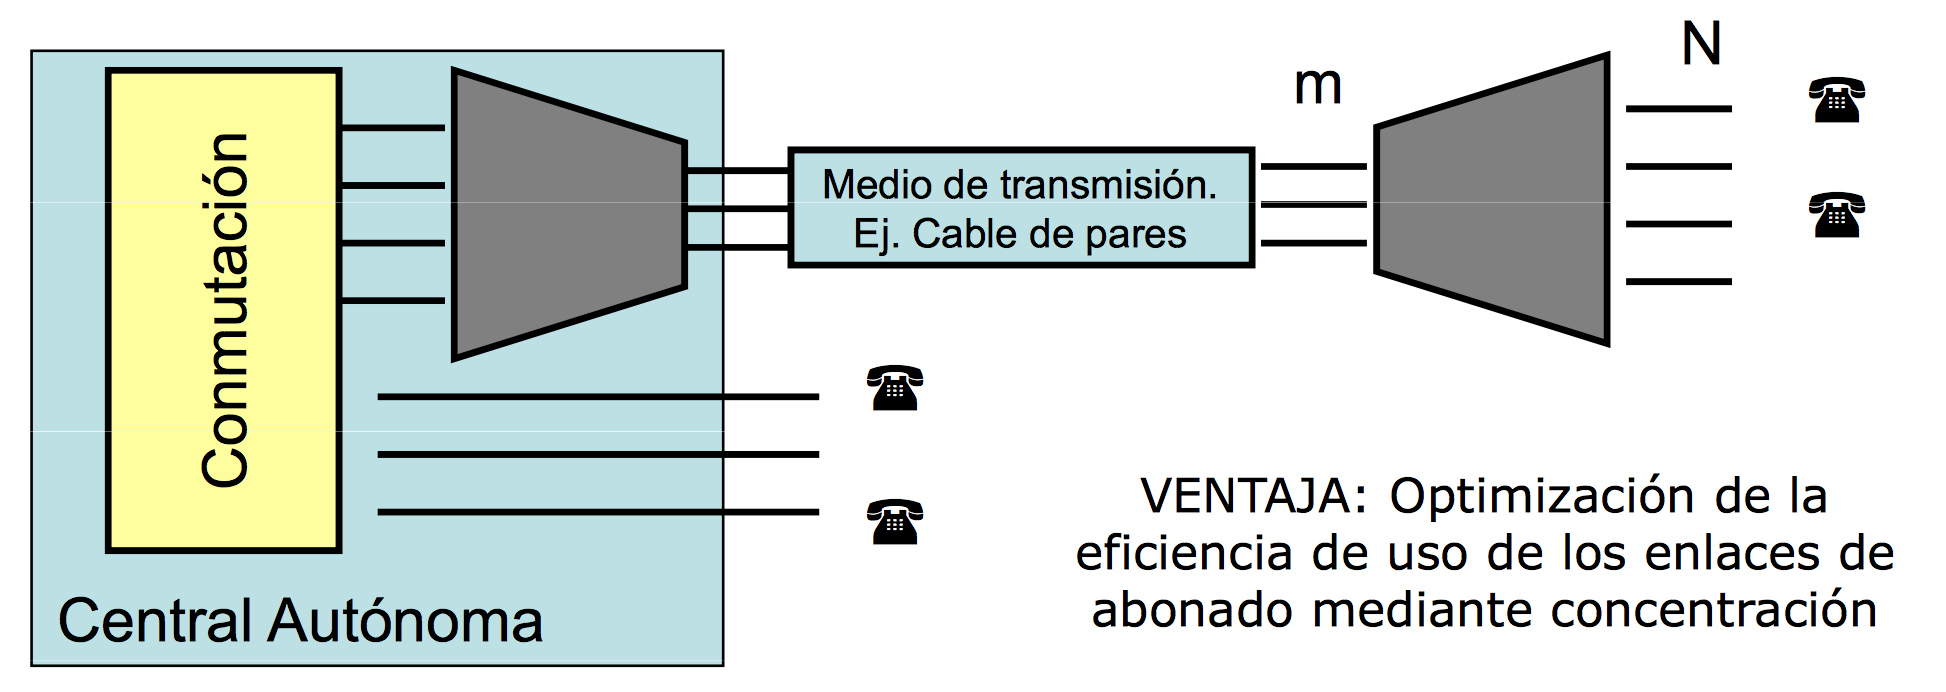
\includegraphics[scale=0.2]{images/RedAcceso}
	\end{center}

\textbf{Unidades remotas de abonados}: son equipos con más capacidad de accesos que el concentrador, están conectados a la central autónoma mediante sistemas MIC por cable o bien enlaces de fibra, su funcionamiento es más autónomo que en el caso de los concentradores y tienen capacidad de conmutación para los enlaces locales.

	\begin{center}
		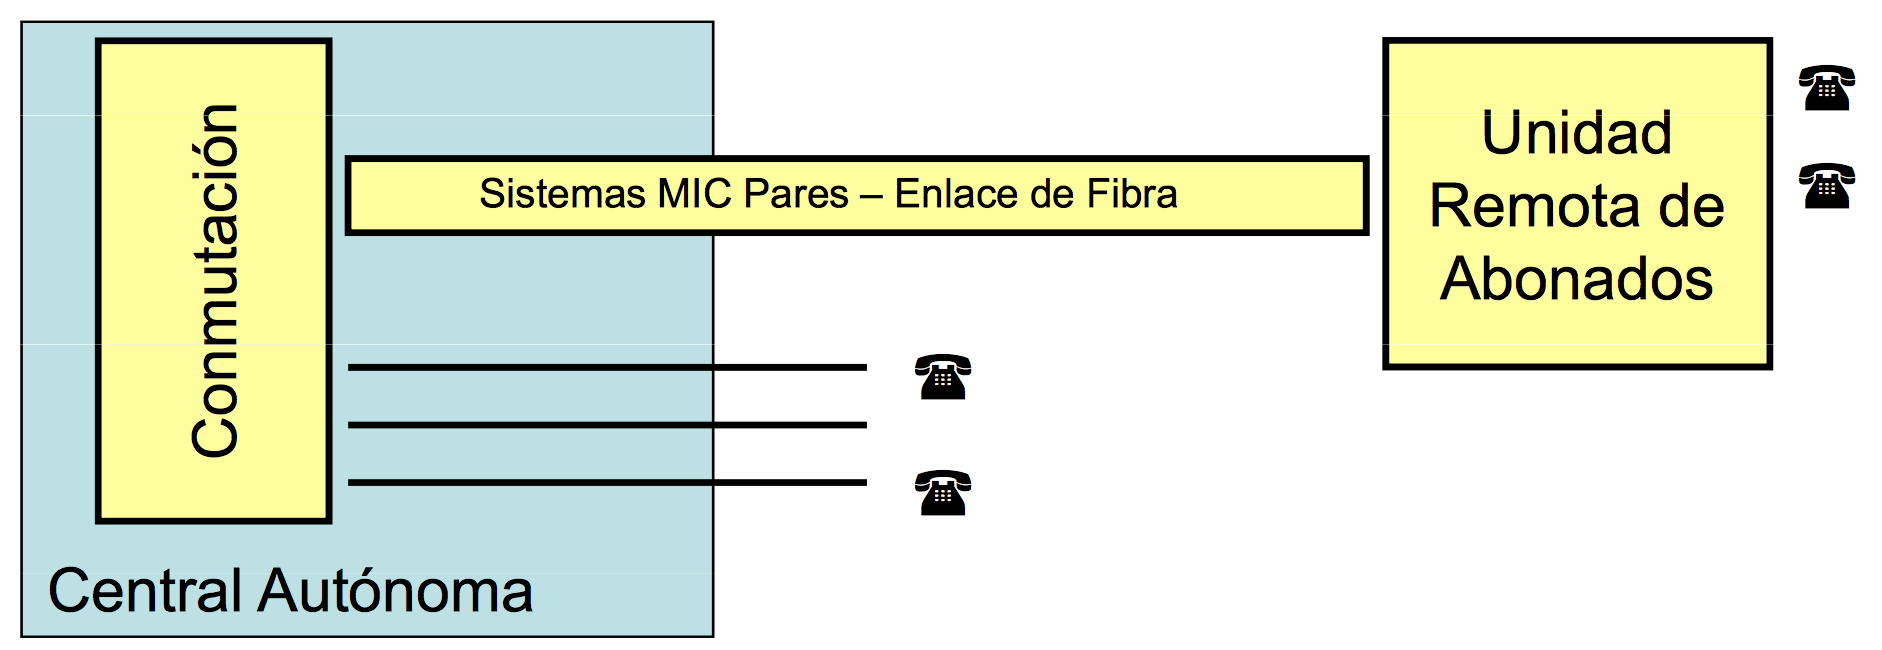
\includegraphics[scale=0.2]{images/RDI}
	\end{center}
		
\subsection{Terminal Telefónico}

\subsubsection{Transmisores y Receptores}

El primer sistema basado en un transmisor, un receptor y una batería dispuestos en serie funcionaba por le principio de resistencia variable. El problema era la potencia del transmisor ya que no existían amplificadores. En la actualizad el transmisor es un micrófono de carbón (no lineal y muy sensible).

\subsubsection{El bucle de Abonado}

El \textbf{bucle de abonado} es una conexión física con la central telefónica, inicialmente era un único hilo (aprovechando la tierra) y actualmente son dos hilos (cable de pares). Inicialmente nació como líneas dedicadas entre dos usuarios, posteriormente fueron líneas de conmutación manual (centralitas) y finalmente son centrales de conmutación (strowger).

\subsubsection{La Bobina de Inducción}

Inicialmente eran un transmisor y un receptor en serie. Tenían \textbf{problemas} como la impedancia del altavoz, difícil adaptación de impedancias y la corriente continua que circulaba a través del receptor reducía su eficiencia. Como \textbf{solución} se utiliza la bobina de inducción, se aíslan los TX y RX facilitando la adaptación y evitando que circule corriente continua por el altavoz.

\subsubsection{El Efecto Local (Sidetone)}

Sigue habiendo un \textbf{problema}, las señales del micrófono se escuchan en el auricular. Hay un tercer camino de alta ganancia entre el altavoz y auricular que hace que el ususario se escuche a sí mismo demasiado alto y tienda a hablar más bajo.
 	
	\begin{center}
		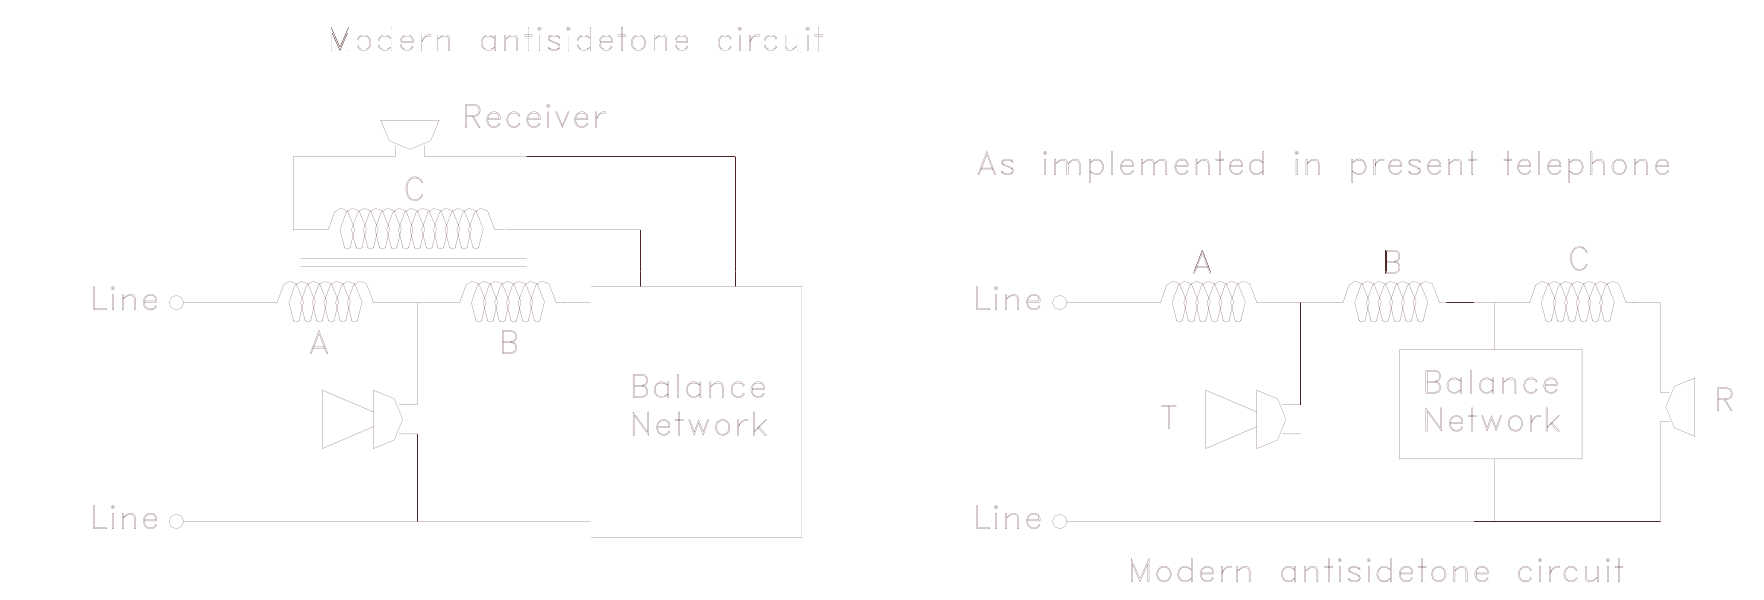
\includegraphics[scale=0.2]{images/Sidetone}
	\end{center}

La adaptación no es perfecta ($Z_{L}$ variable), pero un cierto nivel de sidetone es beneficioso.

\subsubsection{Alimentación y llamada}

La alimentación se realiza desde la central local con $48V$. El consumo de corriente del terminal permite identificar y dar servicio a los usuarios (estados: on-hook y off-hook) \textbf{Insertar Imagen aquí}. El timbre está conectado en paralelo y es de alta impedancia, la señal que se envía a la central es de $75 V_{rms}$ y $50Hz$. 

\subsubsection{Marcación}

\begin{itemize}
	\item \textbf{Por Pulsos/Decamétrica}:
	\item \textbf{DTMF} (\textit{Dual Tone MultiFrequency}):
\end{itemize}

\subsubsection{Otros tipos de terminales}

La ITU define dos tipos de módems:

\begin{itemize}
	\item \textbf{Modems Digitales}: Envía señales G.711 y recibe señales V.34 codificadas con el estándar V.34. Se conecta a una red con conmutación digital con un interfaz digital.
	\item \textbf{Modems Analógicos}: Generan señales V.34 y reciben señales G.711 que han sido decodificadas en una central local de abonado telefónico y preparadas para su envío a través de un bucle de abonado.
\end{itemize}

G.711 - Pulse Code Modulation (PCM) of voice frequencies\\
V.34 - A modem operating (up to 33.600 bit/s) for use in 2-wire analog PSTN

	\begin{center}
		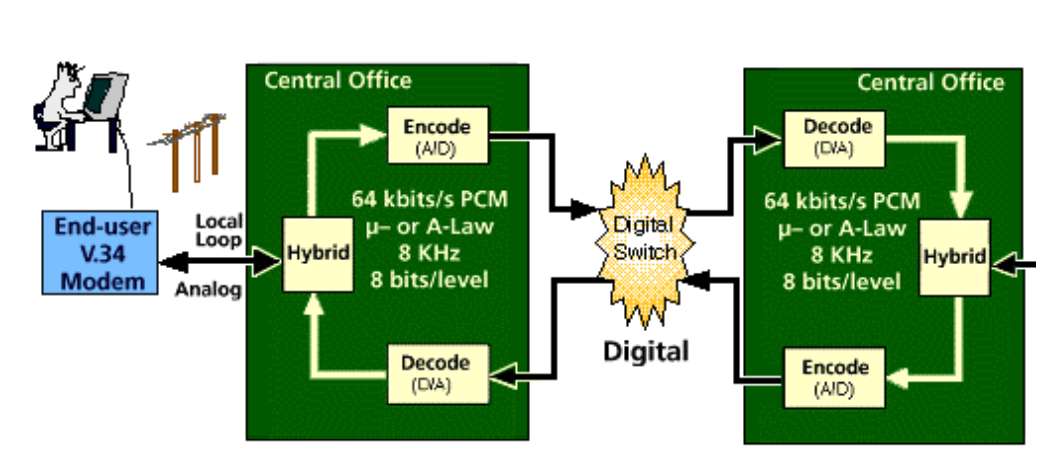
\includegraphics[scale=0.2]{images/SpecsModem}
	\end{center}

Los módems tienen distintas especificaciones que varían según las redes.

\begin{itemize}
	\item V.26 - 2400 bps para uso en líneas alquiladas a 4 hilos
	\item V.27 - 4800 bps para uso en líneas alquiladas
	\item V.27ter - 4800/2400 bps para uso genérico en la red telefónica conmutada
	\item V.29 - 9600 bps para uso en líneas alquiladas punto a punto a 4 hilos
	\item V.34 - 33600 bps para uso genérico en la red telefónica conmutada
	\item V.90 - 56000 bps en el enlace descendente y hasta 33600 bps para el ascendente. Uso genérico en la red telefónica conmutada
\end{itemize}

\textbf{Funciones} de un modem:

	\begin{enumerate}
		\item \textbf{Circuitos para compatibilizar la señalización RDI}: Descolgado, marcado y detección de tono marcado.
		\item \textbf{Circuitos de envío de la señal de datos} en la banda de frecuencias vocal
		\item \textbf{Transmisión a cuatro hilos equivalentes}: Diferentes portadoras en cada sentido e inclusión de filtros para minimizar interferencias.
	\end{enumerate}
	
	\begin{center}
		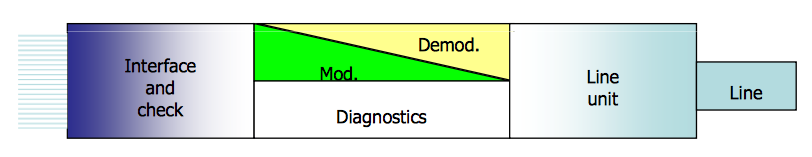
\includegraphics[scale=0.2]{images/FuncModem}
	\end{center}
	
\subsubsection{Operación de un Modem}

El módem receptor espera en answer mode, en el otro extremo espera en call mode y se simula el off-hook escuchando el tono de invitación a marcar y se envían pulsos o tonos para marcar. El modem en modo answer detecta las señales de llamada, simula el off-hook y envía una portadora. El modem en modo llamada envía una portadora y se intercambian los datos ambos.

\subsubsection{Módem V.34}

Permite mayor número de bits por símbolo y permite modulación QAM transmitiendo información en la amplitud y en la fase, incluye códigos de corrección y permite compresión. Estos módems se diseñaron para optimizar la situación en la que ambos lados de la comunicación eran analógicos.

	\begin{center}
		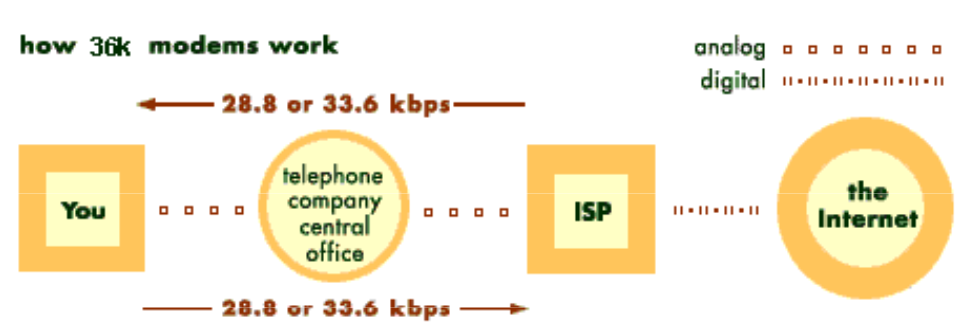
\includegraphics[scale=0.2]{images/ModemV34}
	\end{center}

Este tipo de módems está limitado por el ruido de cuantificación. El estándar V34 no tiene en cuenta la arquitectura real de la conexión entre la red telefónica y el proveedor de acceso a internet, siendo el bucle local la única parte analógica de la transmisión, el ruido de cuantificación sólo está presente en la parte del enlace ascendente.

\subsubsection{Módem V90}

Estándar doméstico desde 1998, el principio de funcionamiento se basa en que el ISP tiene una conexión digital con la central local. Por lo tanto se asume que solo existe una conversión analógico-digital en el camino hasta el ISP.

	\begin{center}
		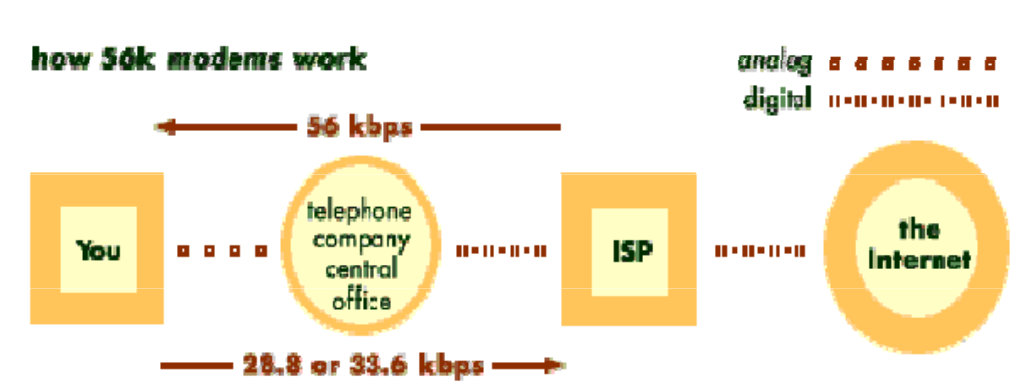
\includegraphics[scale=0.2]{images/ModemV90}
	\end{center}


\subsubsection{Comunicaciones de Facsímil a través de la RTB}

Los terminales de facsímil siguen estándares de la ITU-T. Los faxes se dividen en varios grupos según si el escaneado es digital y su velocidad de transmisión.

\subsection{Bucle de Abonado}


\subsubsection{Introducción}

Medio físico que une la red telefónica con el terminal de abonado. En la RDI este acceso es analógico y basado en cable de pares, representa gran parte del coste de una red.

\subsubsection{Distribución entre la central y el abonado}

El interfaz con la red telefónica: La centrla local

	\begin{center}
		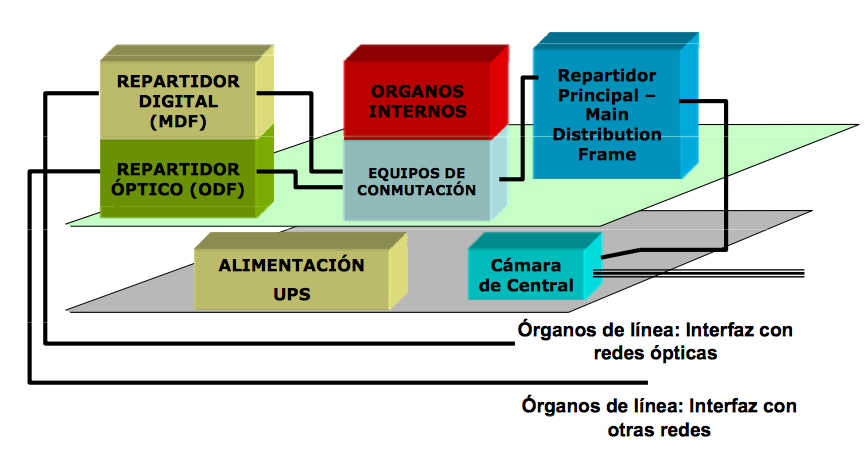
\includegraphics[scale=0.2]{images/CentralLocal}
	\end{center}

Esquema de distribución de cable de pares

	\begin{center}
		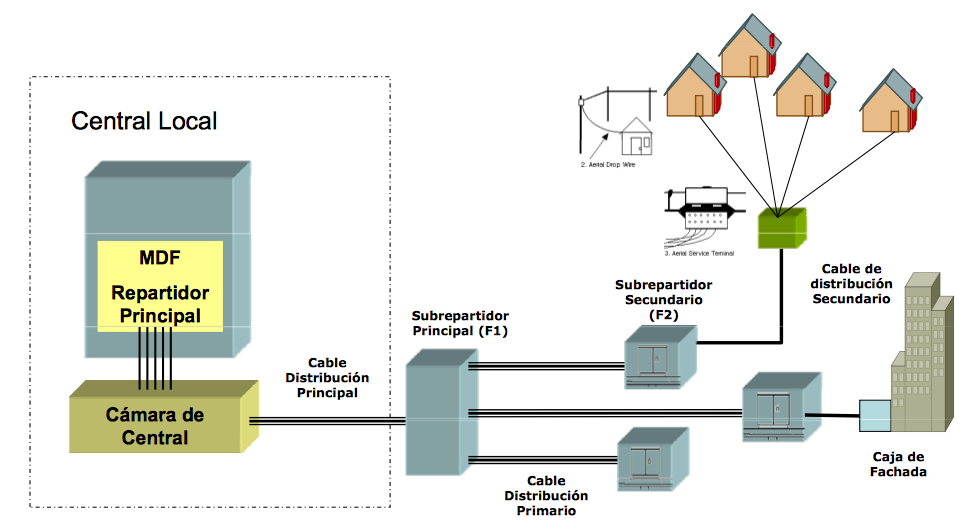
\includegraphics[scale=0.2]{images/Distribucion}
	\end{center}	

Bridged - Taps


	\begin{center}
		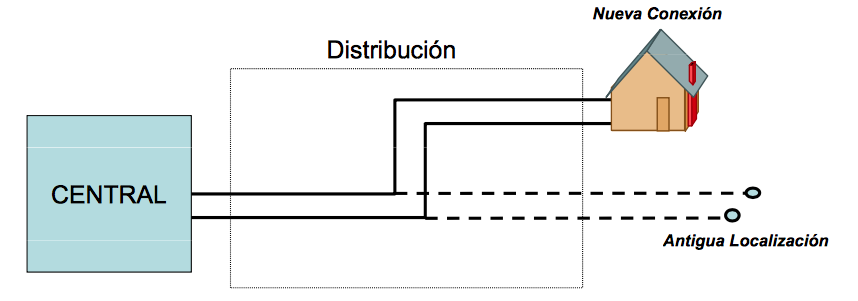
\includegraphics[scale=0.2]{images/Taps}
	\end{center}
	
Extensión en circuito abierto conectado en paralelo a un bucle de abonado, puede originarse en un cambio de conexión (nueva localización). Permite dar flexibilidad en las instalaciones telefónicas. Produce desadaptación de impedancias, reflexiones (problema en los equipos de línea de la central y el abonado). Es dañino en altas frecuencias (ADSL).

\subsubsection{Elementos básicos de la instalación}

\subsubsection{Características típicas del bucle de abonado}

Los cables se clasifican según su galga (diámetro), según su categoría permiten se establece su velocidad de transmisión y su aplicación varía. La distancia máxima del bucle del abonado está limitada por \textbf{limitación óhmica} y \textbf{limitación por pérdidas (atenuación)}.

\subsubsection{Centrales locales: Interfaz con el bucle de abonado}

	\begin{center}
		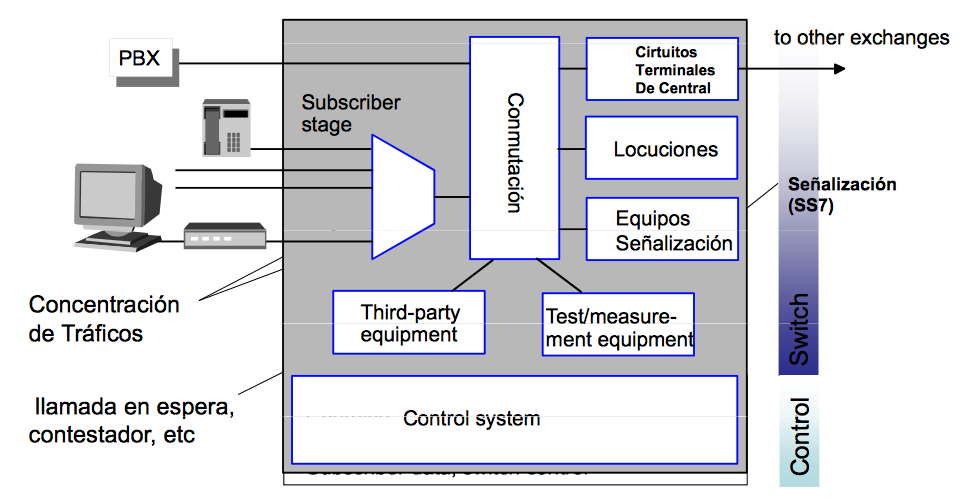
\includegraphics[scale=0.2]{images/CentralFuncional}
	\end{center}
	
La central local tiene como \textbf{funciones}: \textbf{funciones de mantenimiento} en la que supervisa las líneas de abonado y los enlaces y \textbf{funciones de operación} en las que maneja datos administrativos y datos estadísticos.

	\begin{center}
		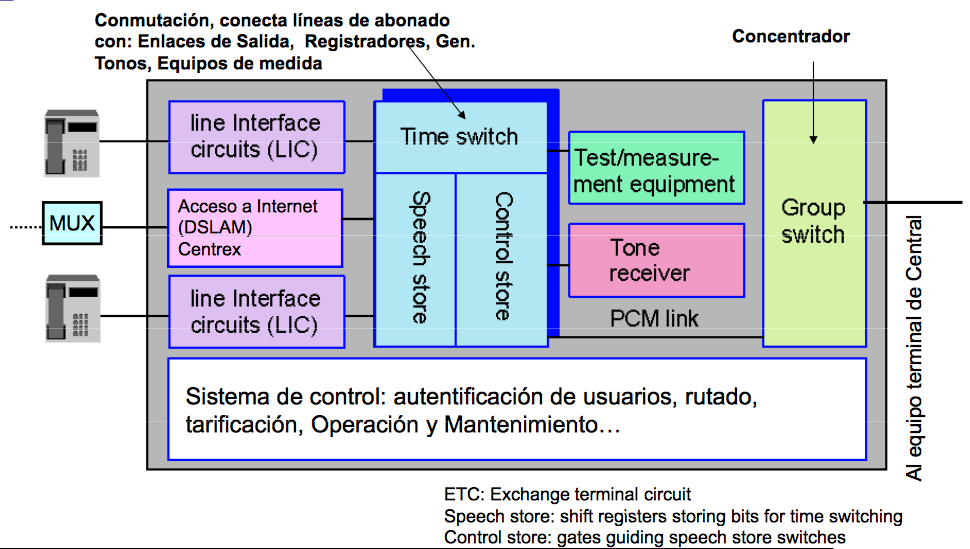
\includegraphics[scale=0.2]{images/CentralFuncional2}
	\end{center}

El interfaz con la red telefónica

	\begin{center}
		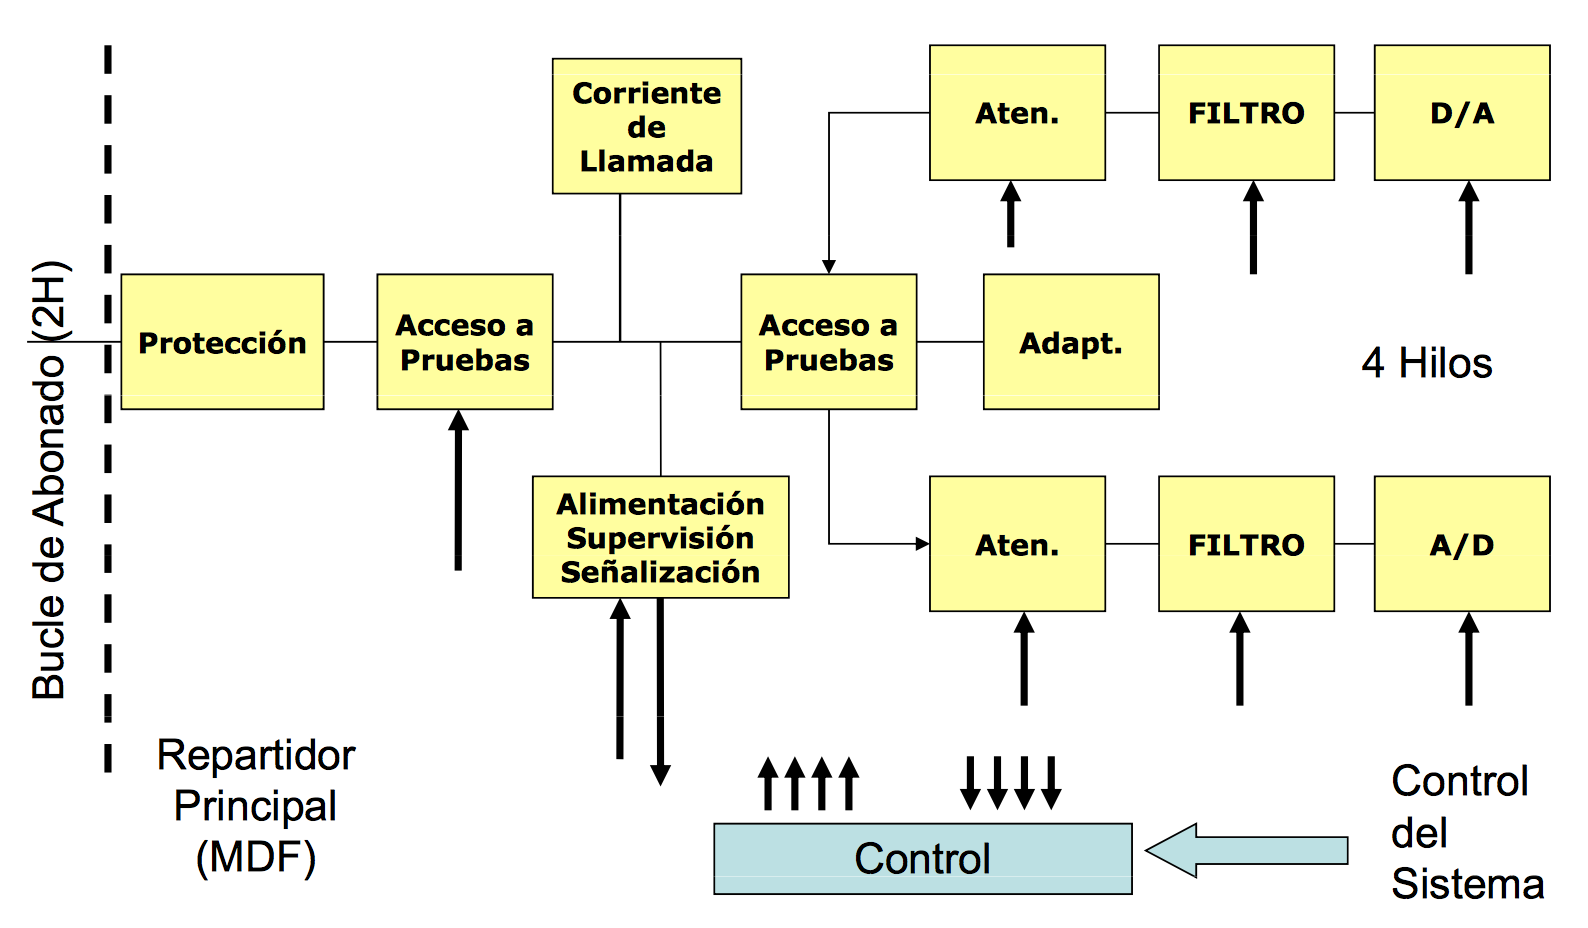
\includegraphics[scale=0.2]{images/InterfazRed}
	\end{center}

\subsubsection{Perturbaciones en el bucle de abonado}

La \textbf{bobina híbrida} permite separar los canales de ida y vuelta. Las conexiones entre abonados son a dos hilos y las conexiones entre centrales son a cuatro hilos. Al ser elemenots ideales, en las redes telefónicas se ocasionan los problemas de ECO y CANTO.

	\begin{center}
		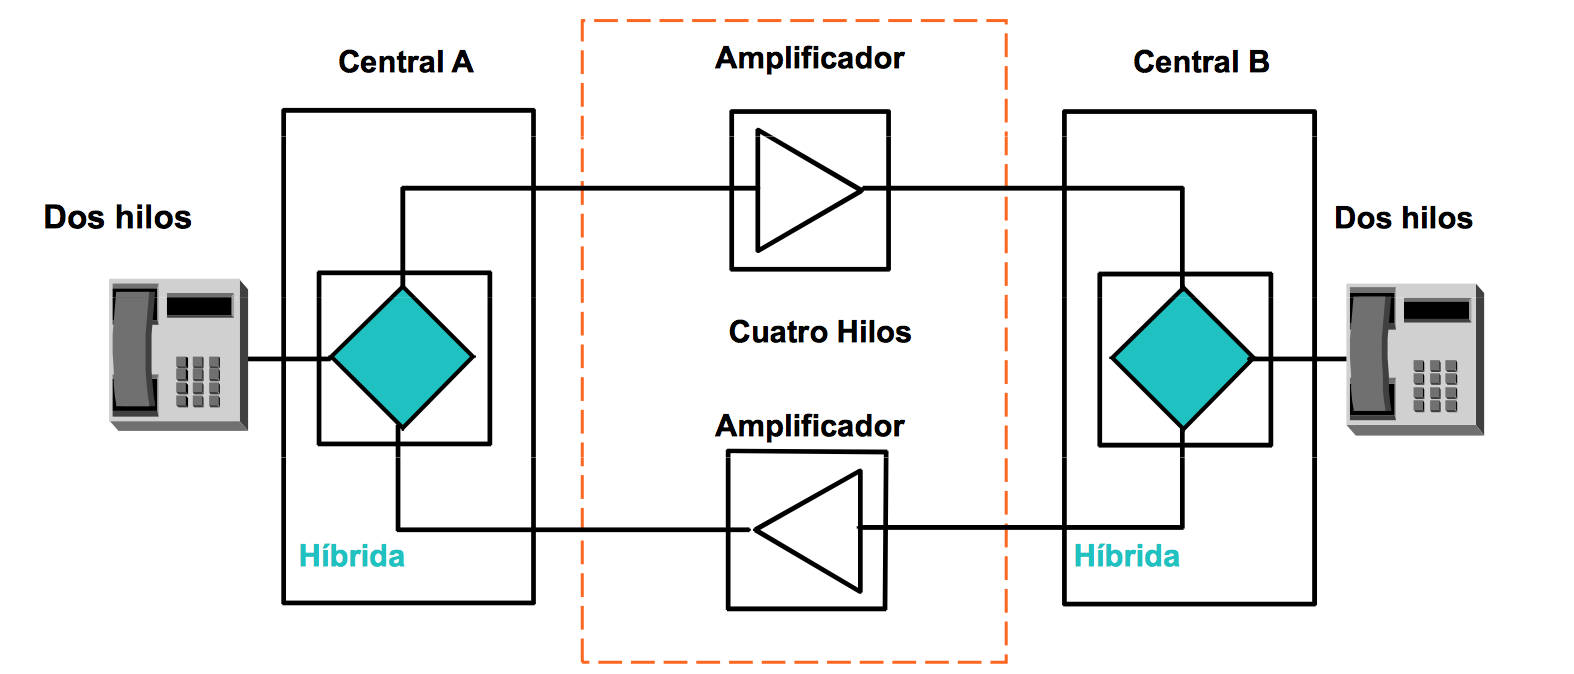
\includegraphics[scale=0.2]{images/BobinaHibrida}
	\end{center}
	
\textbf{Pérdidas de retorno}:

	\begin{equation*}
		A_{R} =  20 \cdot \log(\left| \frac{1}{\rho} \right| ) = 20 \cdot \log \left| \frac{Z_{L} + Z_{E}}{Z_{E} - Z_{L}} \right|
	\end{equation*}

\textbf{Atenuación Transhíbrida}:

	\begin{equation}
		A_{TH} = 2 \alpha + A_{R}
	\end{equation}•
	
\textbf{Estudio de la Inestabilidad}:	
	
Pérdida entre extremos a 2 hilos: $T = 2 \alpha + L - G$

Margen de estabilidad $S = \frac{M}{2}$. El bucle a cuatro hilos será estable si no tiene ganancia, es decir, si $M = 0$. Habitualmente $S = 3 dB$.	
	
En la bobina híbrida aparecen dos tipos de \textbf{eco}:

	\begin{itemize}
		\item \textbf{Eco del hablante}: el hablante escucha un eco de su propia voz
		\item \textbf{Eco del oyente}: el oyente escucha un eco de la señal que escucha
	\end{itemize}
	
Para solucionar estos problemas se utilizan dos componentes. \textbf{NES} (\textit{Network Echo Supressor}) anula la línea de transmisión cuando se detecta la señal recibida. Es equivalente a una comunicación semi-dúplex.
	
	\begin{center}
		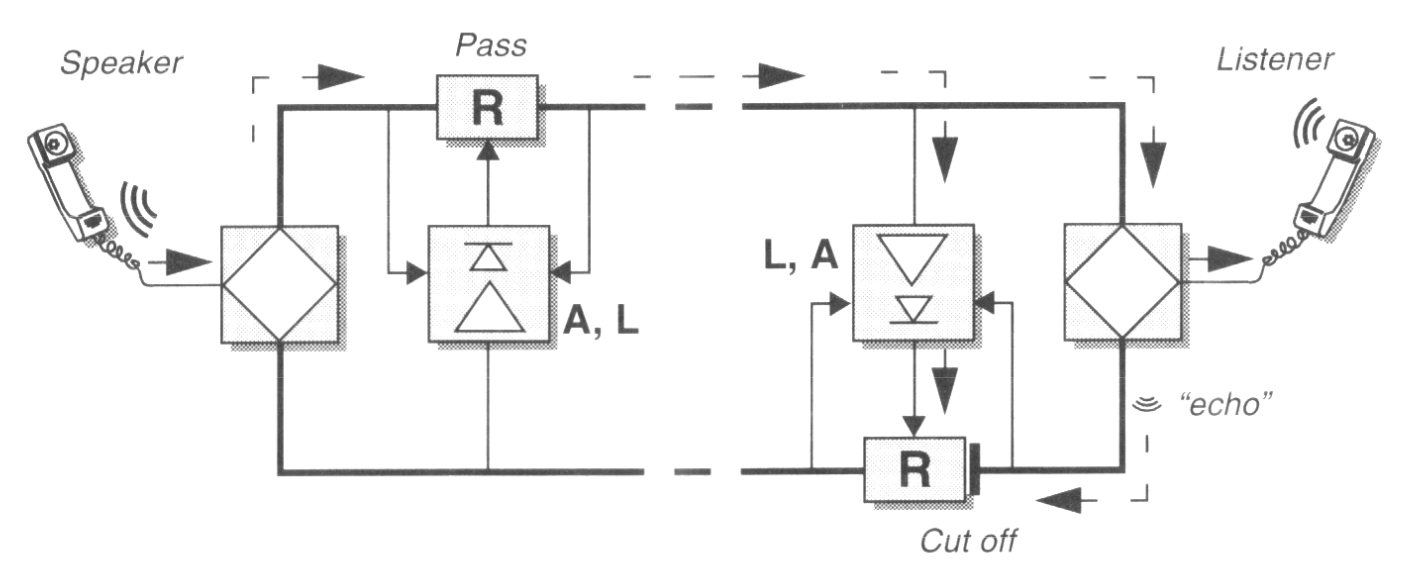
\includegraphics[scale=0.2]{images/NES}
	\end{center}
	
El \textbf{NEC} (\textit{Network Echo Canceller}) elimina en la rama de transmisión la señal de eco calculada a partir de la rama de recepción

	\begin{center}
		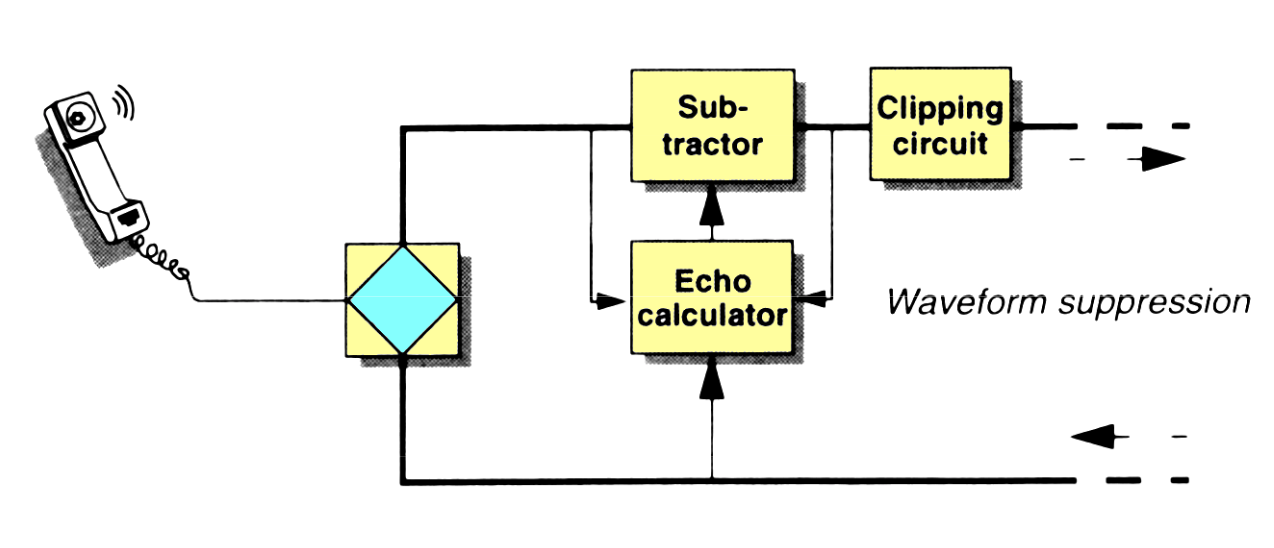
\includegraphics[scale=0.2]{images/NEC}
	\end{center}

\textbf{Interfaces PSTN e ISDN en una central local}. ISDN es Inegrated Service Data Network y PSTN Public Switched Telephone Network.

	\begin{center}
		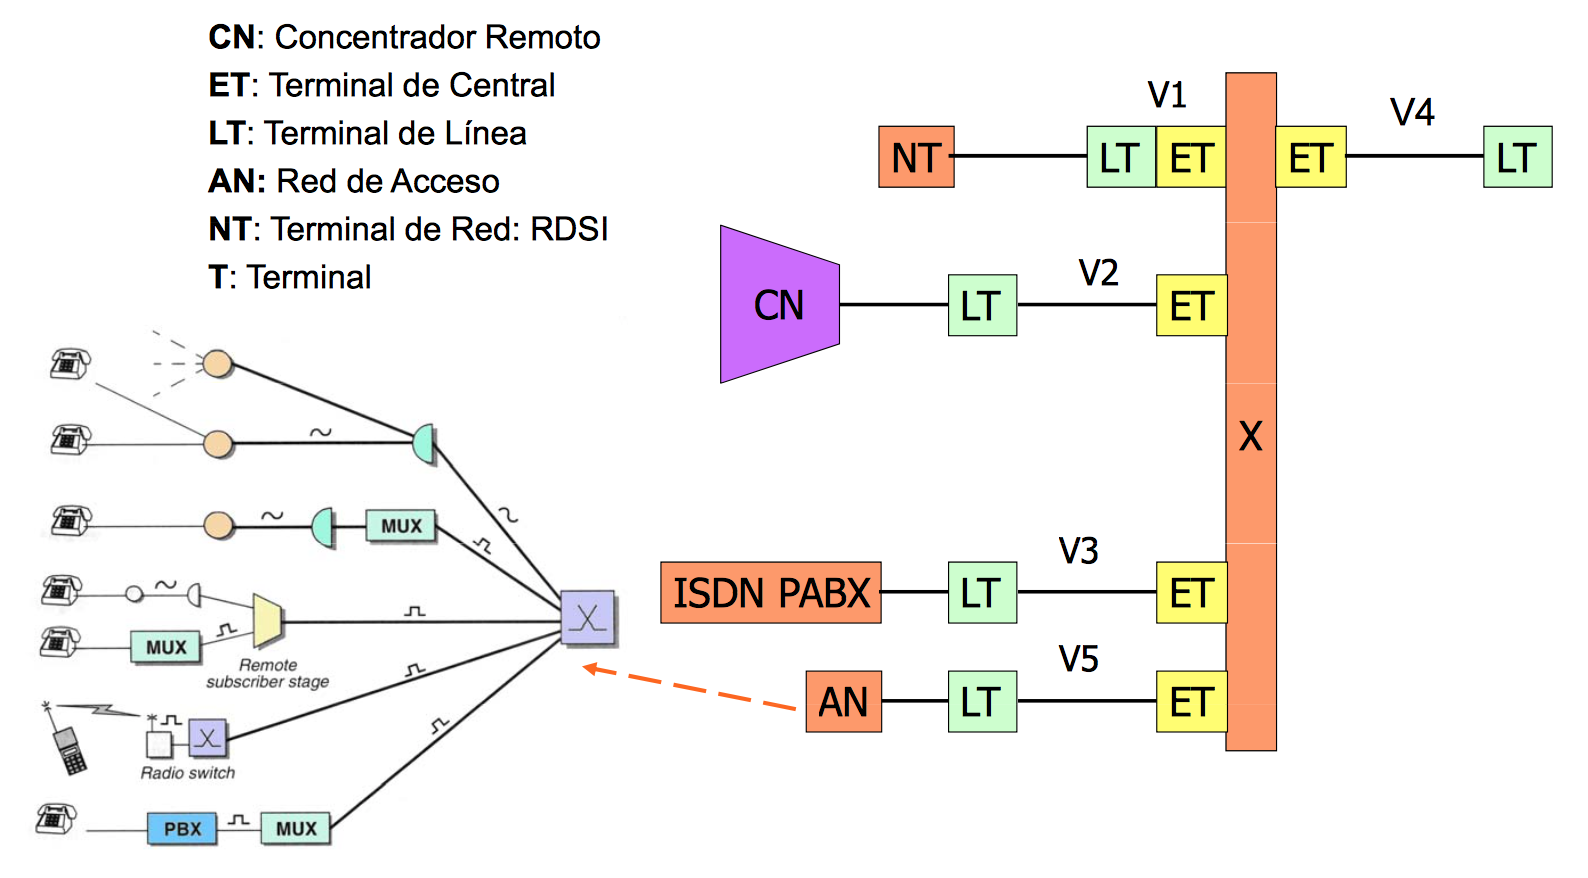
\includegraphics[scale=0.2]{images/ISDN}
	\end{center}

\textbf{Interfaz V1} acceso básico para la RDSI, sus funciones básicas son: $2B + D$ ($2x64 kbps + 16 kbps$ canalización), temporización y sincronismo de trama, activación y desactivación del terminal de línea, operación y mantenimiento, alimentación... \textbf{V2 Interfaz para la conexión con concentradores}: 2048 kbit/s, $30B + D$. \textbf{V3 similar a V2 pero pensado para interfaz con centralitas (PABX)}: $30B + D$ a 2048 kbit/s y también $23B+D$ a 1544 kbit/s.



\subsubsection{DLC (Digital Loop Carriers)}



\subsection{xDSL}

\subsection{HFC y redes de fibra}


\subsection{Acceso Vía Radio}


\subsection{Sistemas PCM}

%%%%%%%%%%%%%%%%%%%%%%%%%%%%%%%%%%%%%%%%%%%%%%%%%%%%%%%%%%%%%%%%%
% Tema 5

\hrulefill

\section{\underline{Redes Troncales y de Transporte}}

\hrulefill

\subsection{PDH}

\subsubsection{Introducción}

La tecnología PDH (\textit{Plesiochronous Digital Hierarchy}) permite multiplexar en tramas de orden superior afluentes MIC 30+2. Optimiza los recursos en los enlaces transmitiendo el mayor número de canales vocales posibles con el mínimo de recursos. Al ser sistemas digitales, la multiplexación es TDM. PDH consiste en una red en la que los relojes con ``casi'' síncronos, tendrán la misma velocidad pero estarán sujetos a una tolerancia. Existen varios estándares. Es coherente con la diferencia en el proceso de creación de la trama básica MIC.\\

Las jerarquías digitales son la herramienta de transporte de las redes telefónicas digitales.

	\begin{center}
		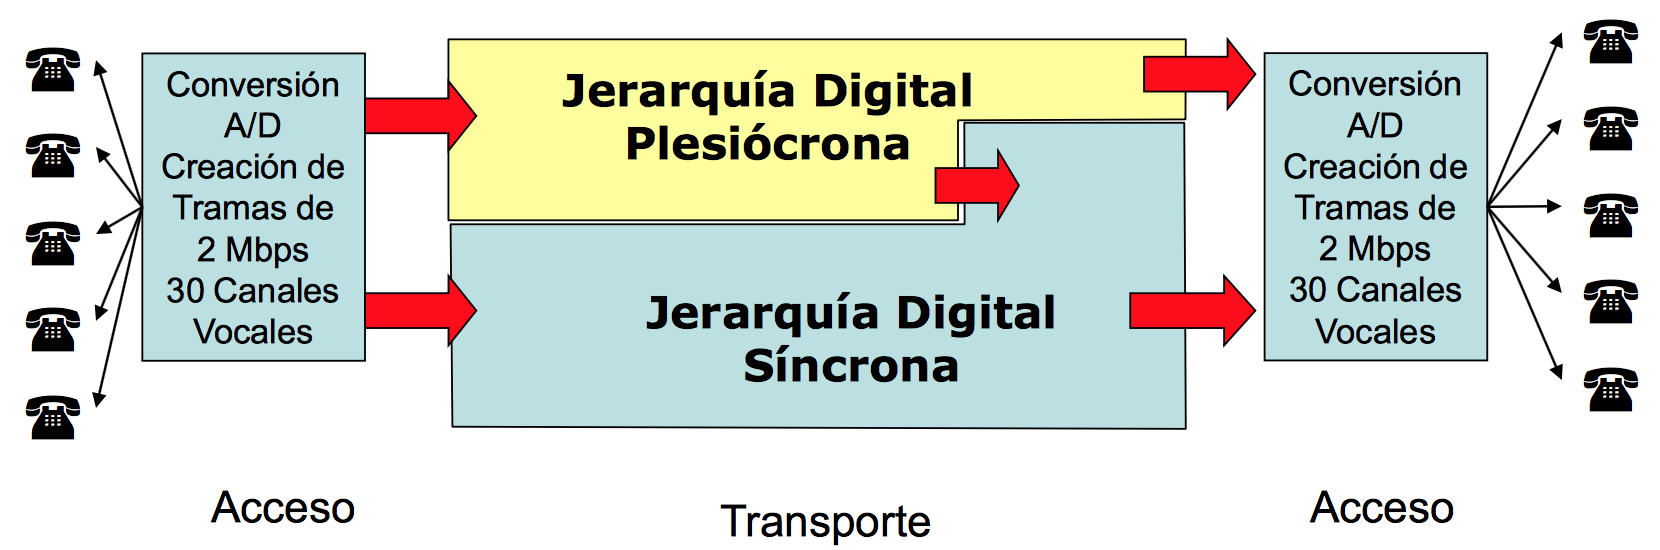
\includegraphics[scale=0.2]{images/Jerarquia}
	\end{center}
	
La UIT especifica los niveles de multiplexación posible y la estructura de las tramas multiplexadas.

	\begin{center}
		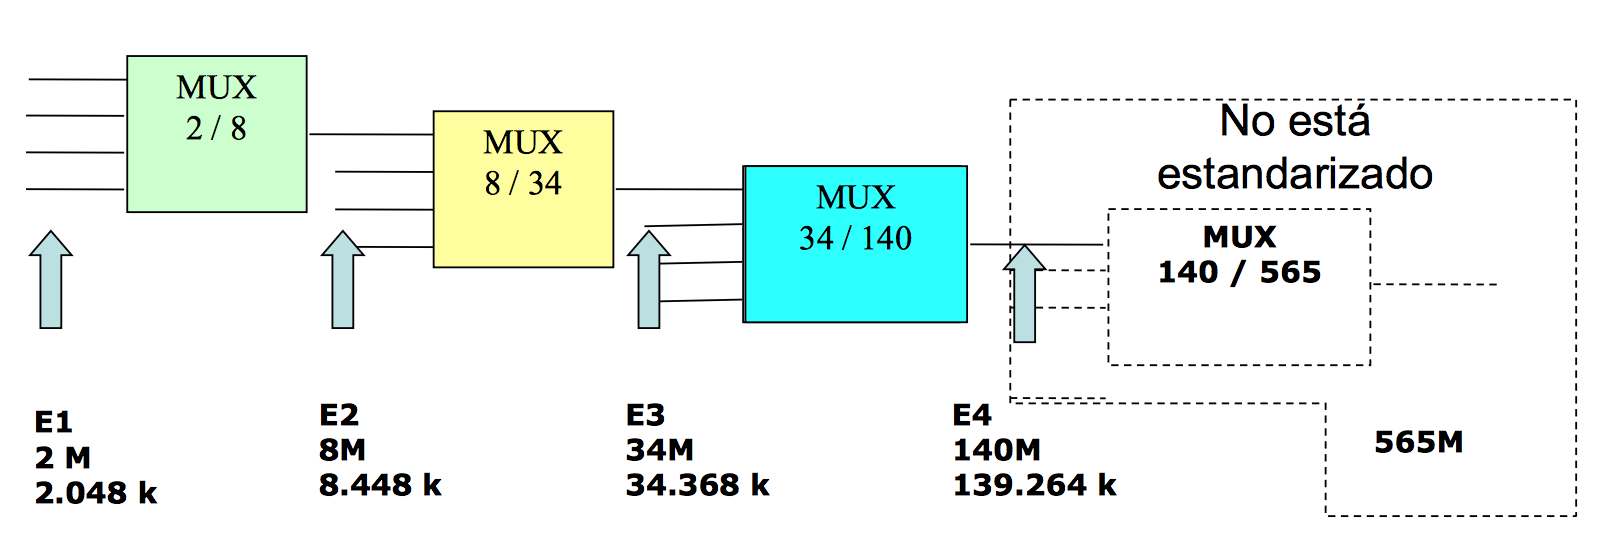
\includegraphics[scale=0.2]{images/NivelesMUX}
	\end{center}

Las señales de entrada a un multiplexor son \textbf{tributarias} o \textbf{afluentes}. La multiplexación se realiza a nivel del bit.

\subsubsection{Velocidades PDH}

	\begin{center}
		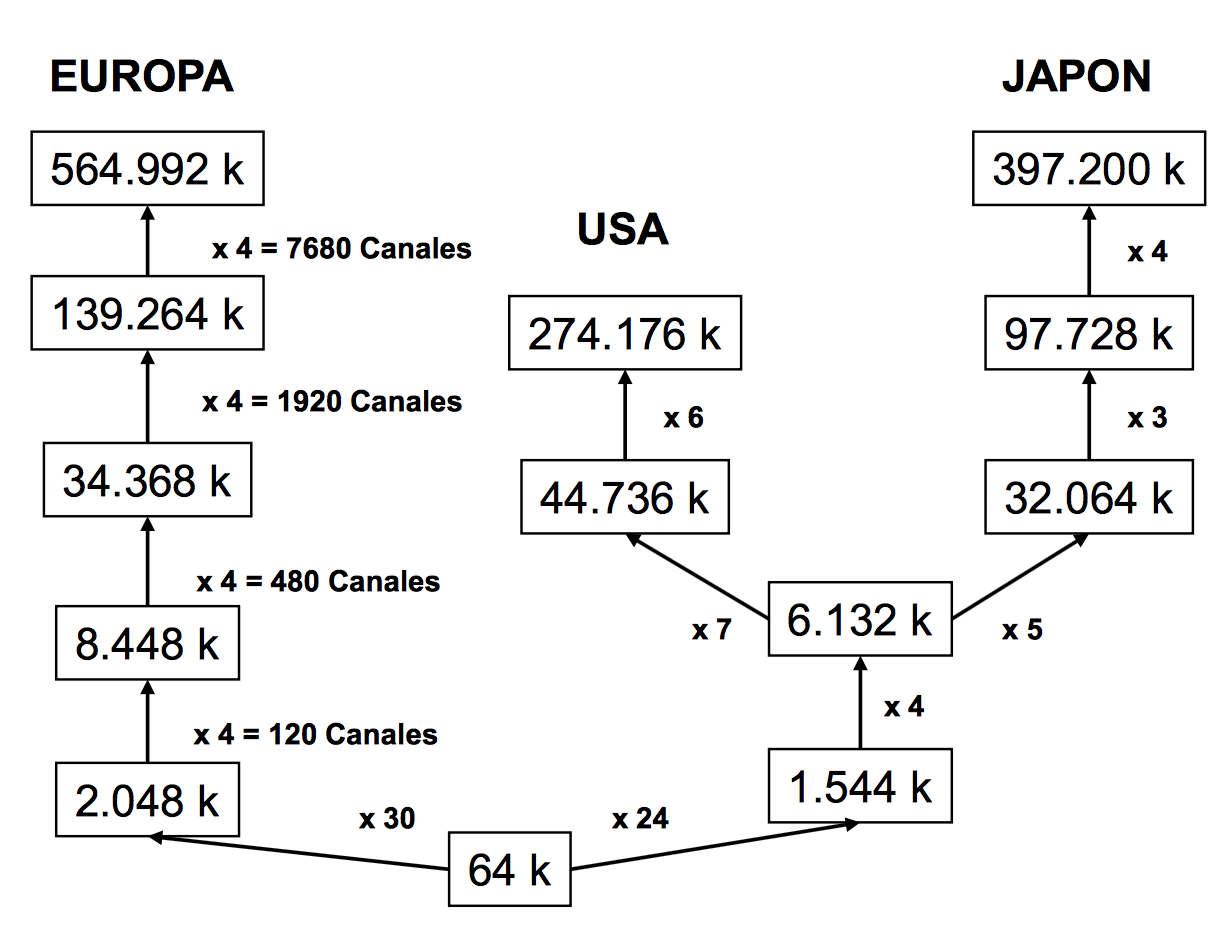
\includegraphics[scale=0.2]{images/VelocidadPDH}
	\end{center}

	\begin{center}
		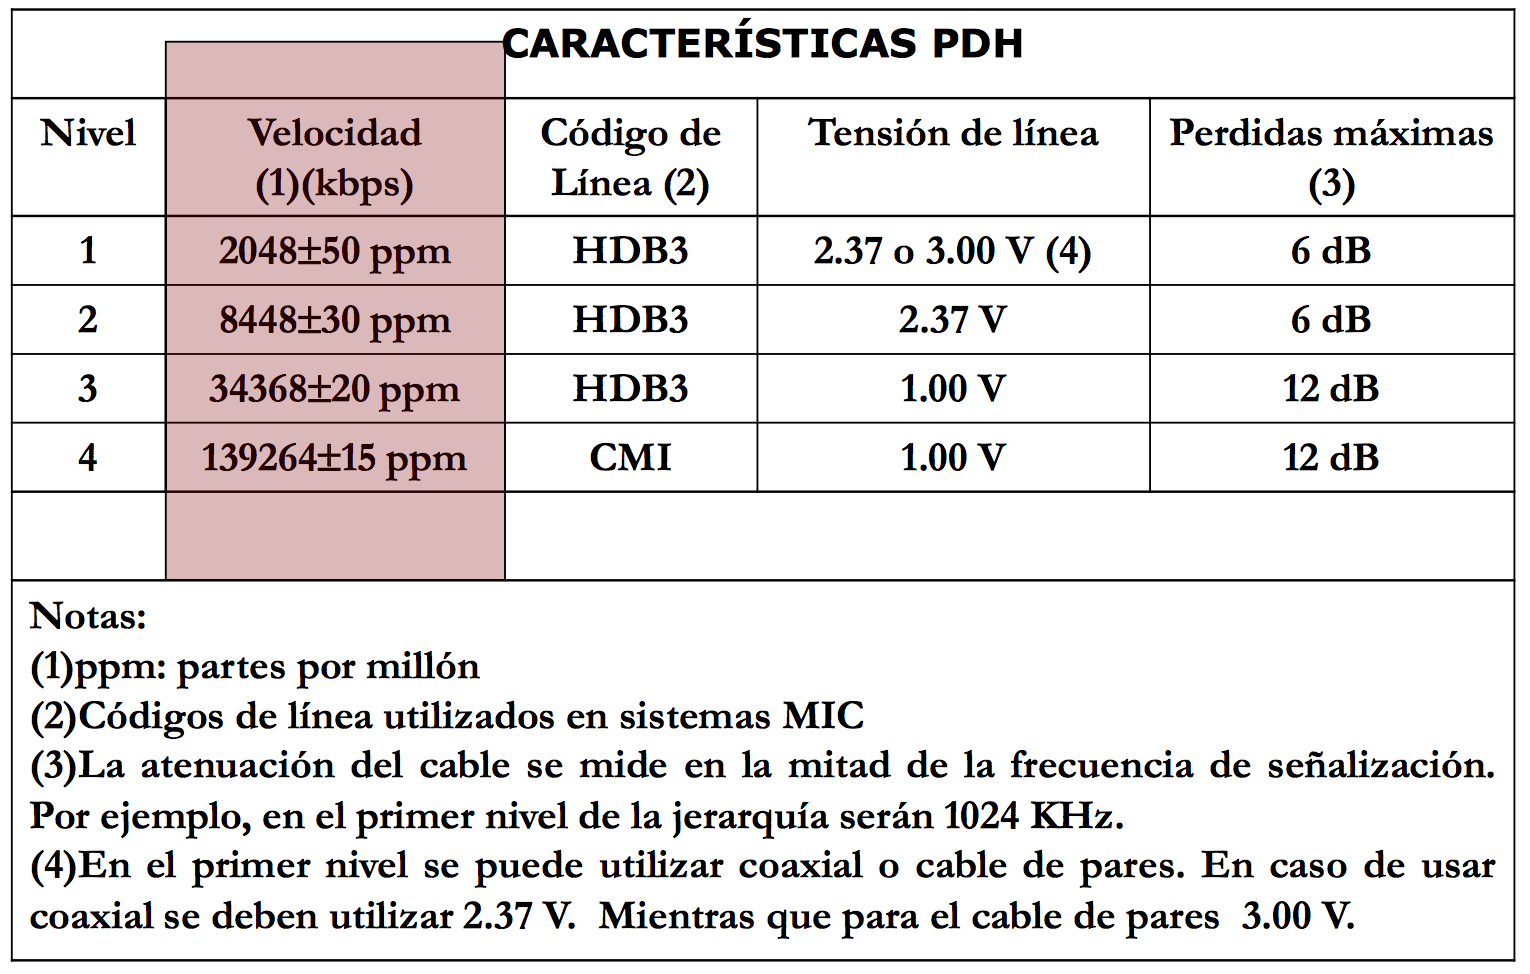
\includegraphics[scale=0.2]{images/CaracteristicasPDH}
	\end{center}	

\subsubsection{Justificación o Relleno}

Los equipos de la red PDH no están sincronizados, utilizan distintos relojes con la misma velocidad pero con tolerancias sobre la velocidad nominal. Esto supone un problema para la multiplexación.

	\begin{center}
		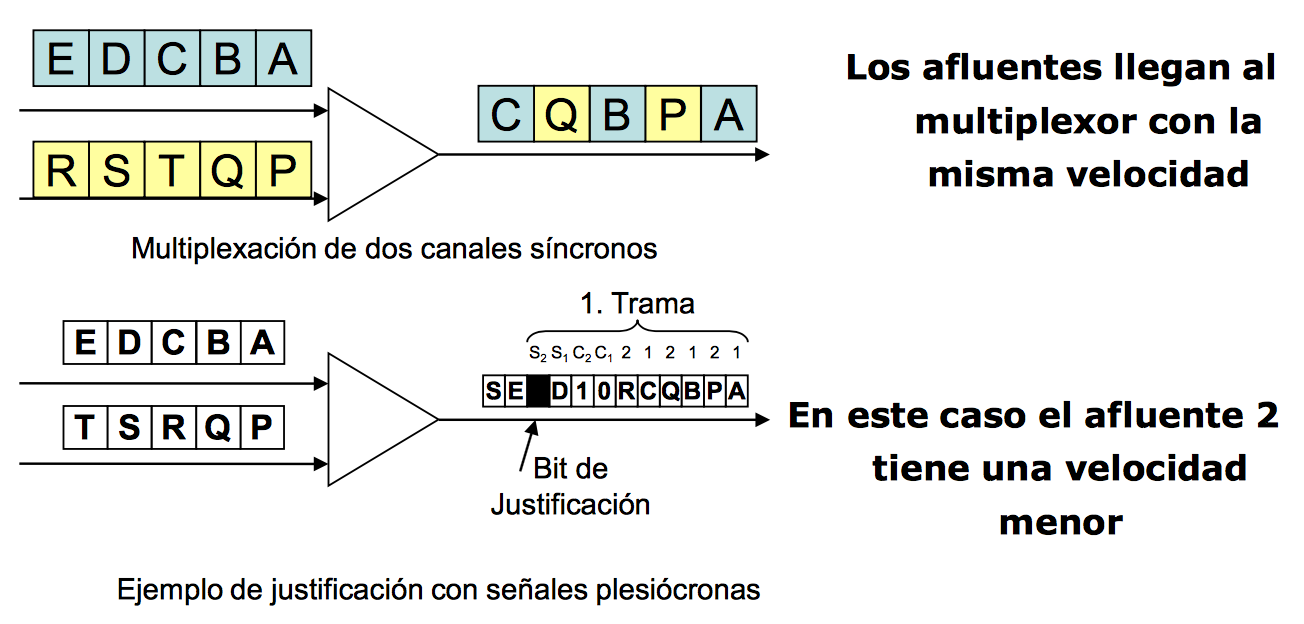
\includegraphics[scale=0.2]{images/JustificacionPDH}
	\end{center}	

Las tramas contemplan espacios para bits de relleno que se pueden utilizar como bits de información si es necesario $\rightarrow$ Justificación positiva
	
	\begin{center}
		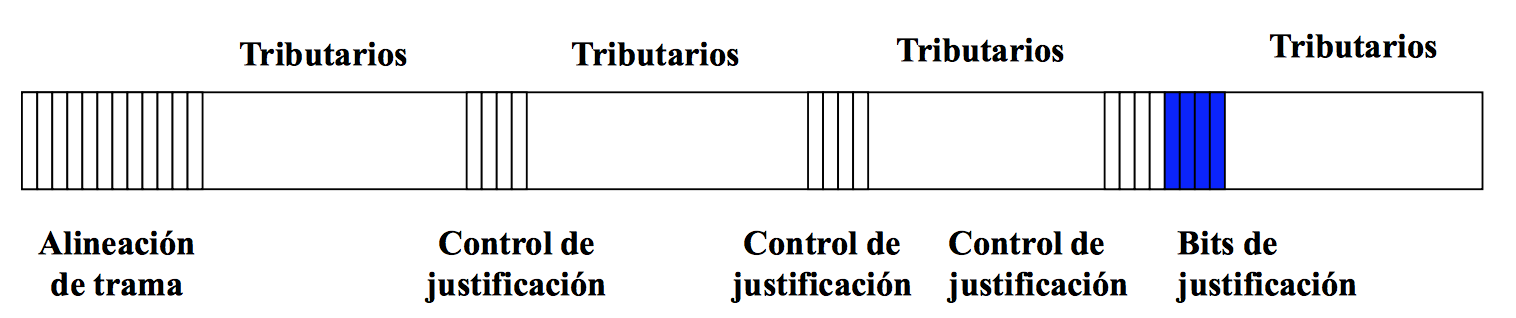
\includegraphics[scale=0.2]{images/Relleno}
	\end{center}	

La técnica de justificación tiene tres variantes: positiva, negativa (supresión de impulsos sobre los afluentes), positiva-nula-negativa (usada en la SDH). Si se ha utilizado justificación en la trama es necesario indicarlo, hay bits de control de justificación sobre qué afluente se ha realizado.

\subsubsection{Estructura de la trama G.742 - 8 Mbps}
	
	\begin{center}
		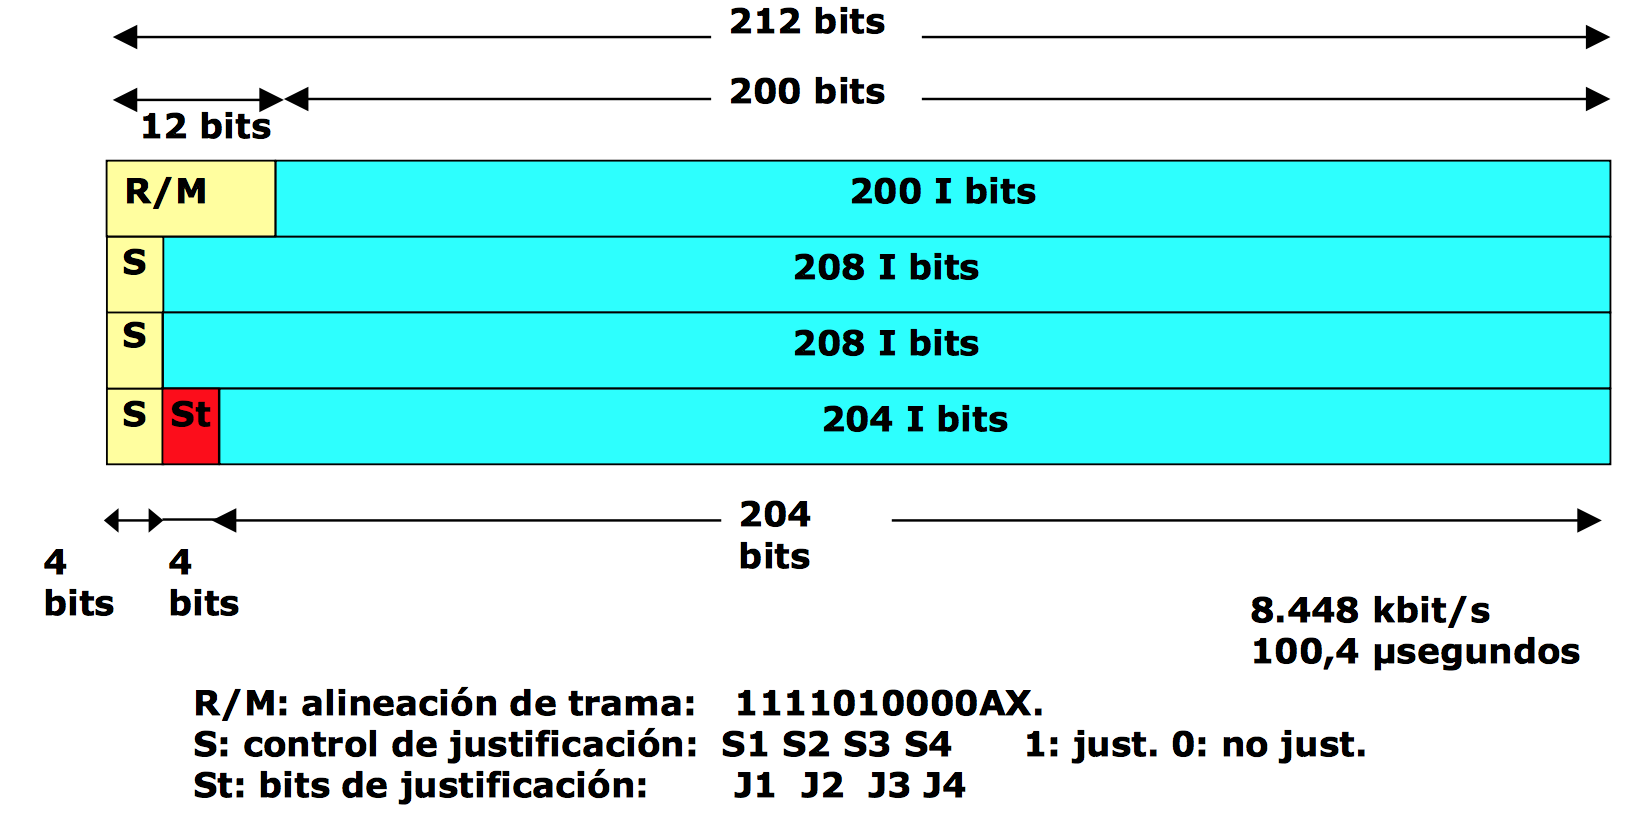
\includegraphics[scale=0.2]{images/TramaG742}
	\end{center}	

\subsubsection{Estructura de las tramas G.751 - 34 Mbps}

	\begin{center}
		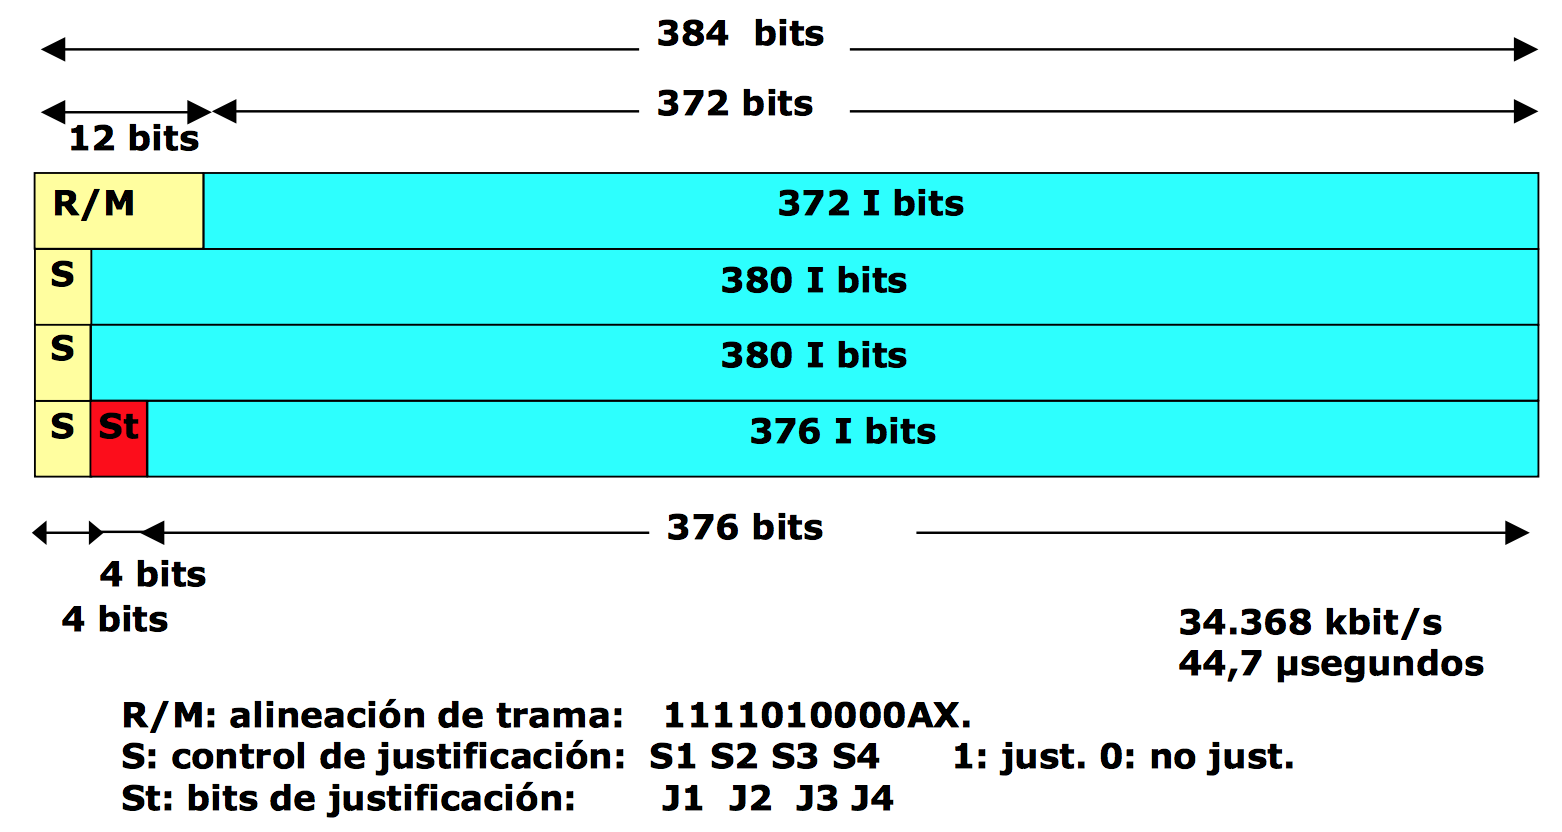
\includegraphics[scale=0.2]{images/TramaG751}
	\end{center}
	
\subsubsection{Estructura de las tramas G.751 - 140 Mbps}

	\begin{center}
		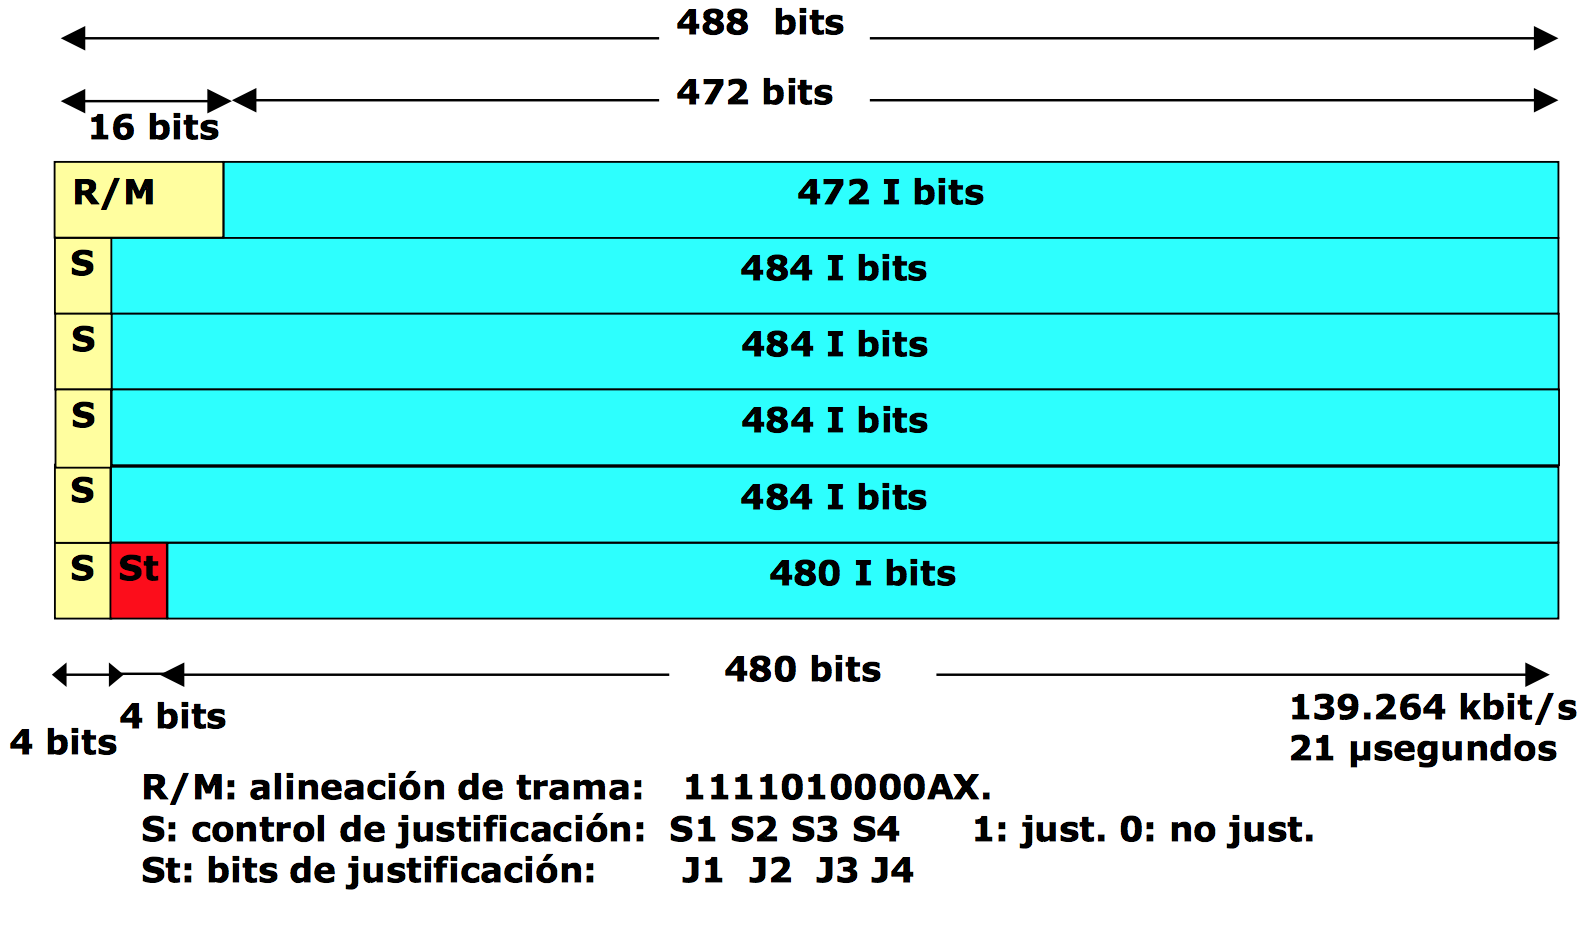
\includegraphics[scale=0.2]{images/TramaG7512}
	\end{center}		

\subsubsection{Velocidades de trama de señales PDH}

\textbf{Tasa Nominal de Justificación}: $\theta = \frac{F_{J}}{F_{A}}$\\
	\quad $F_{A}$: Velocidad de justificación cuando el afluente llega a velocidad nominal\\
	\quad $F_{J}$: Frecuencia Nominal de Justificación

\textbf{Frecuencia de Redundancia}\\
	\quad Frecuencia a la que se insertan los bits de control \\
	\quad Tasa de redundancia $R$
	
\textbf{Relación Nominal de Justificación}: Relación entre la velocidad nominal de justificación  y la velocidad máxima de justificación posible. $g = \frac{F_{J}}{F_{J}^{MAX}}$

\textbf{Frecuencia del Múltiplex}: $F_{M} = N \cdot F_{A} * (1 + \theta) (1 + R)$


\subsubsection{Tipos de Equipos en redes PDH}

\textbf{Terminales de línea}

\textbf{Multiplexores}

	\begin{center}
		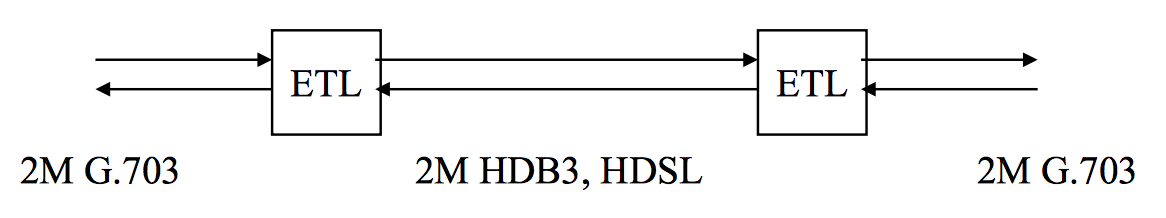
\includegraphics[scale=0.2]{images/Electrico}
	\end{center}	

\textbf{Radio}

	\begin{center}
		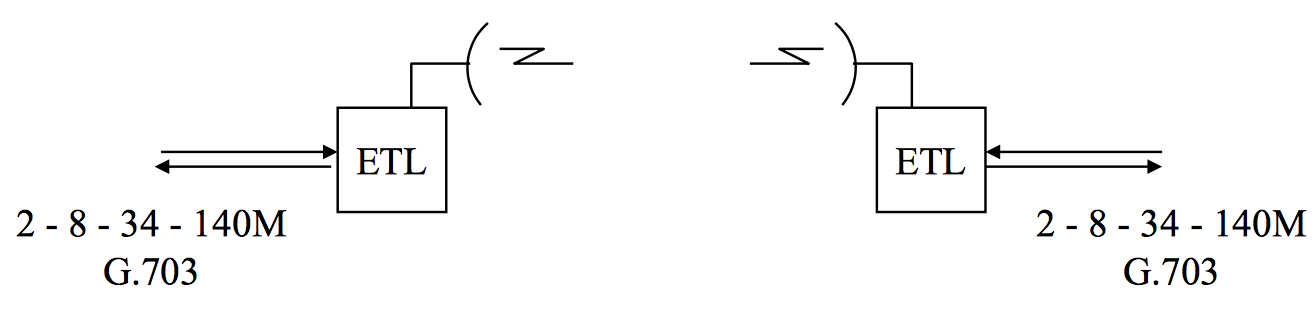
\includegraphics[scale=0.2]{images/Radio}
	\end{center}

\textbf{Optico}

	\begin{center}
		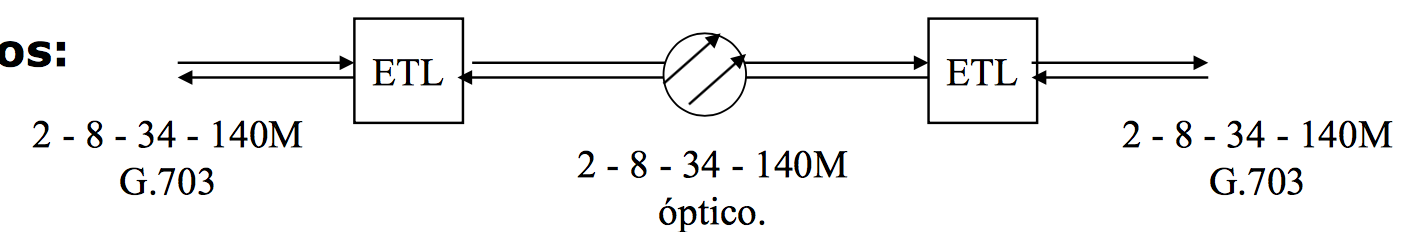
\includegraphics[scale=0.2]{images/Optico}
	\end{center}

\textbf{Multiplexores de acceso: canales de usuario / 2M}

	\begin{center}
		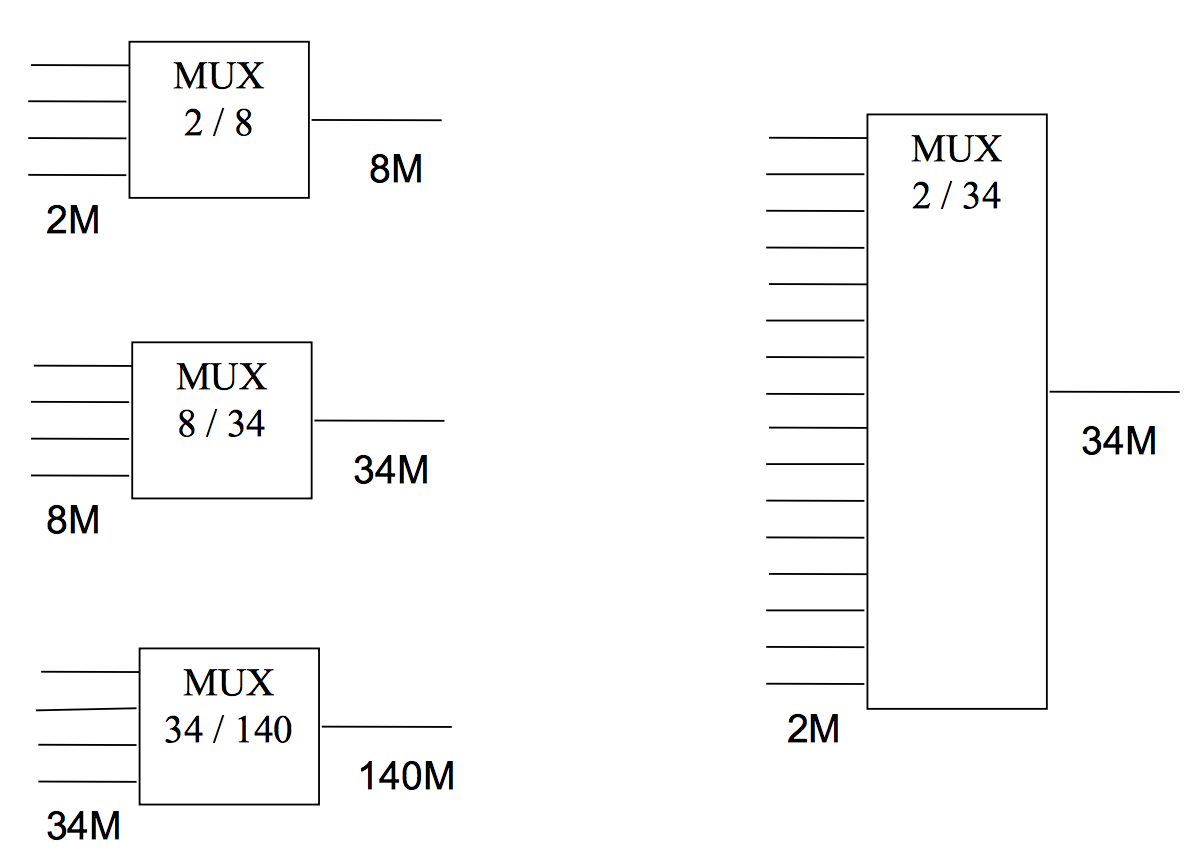
\includegraphics[scale=0.2]{images/Mux}
	\end{center}

	\begin{center}
		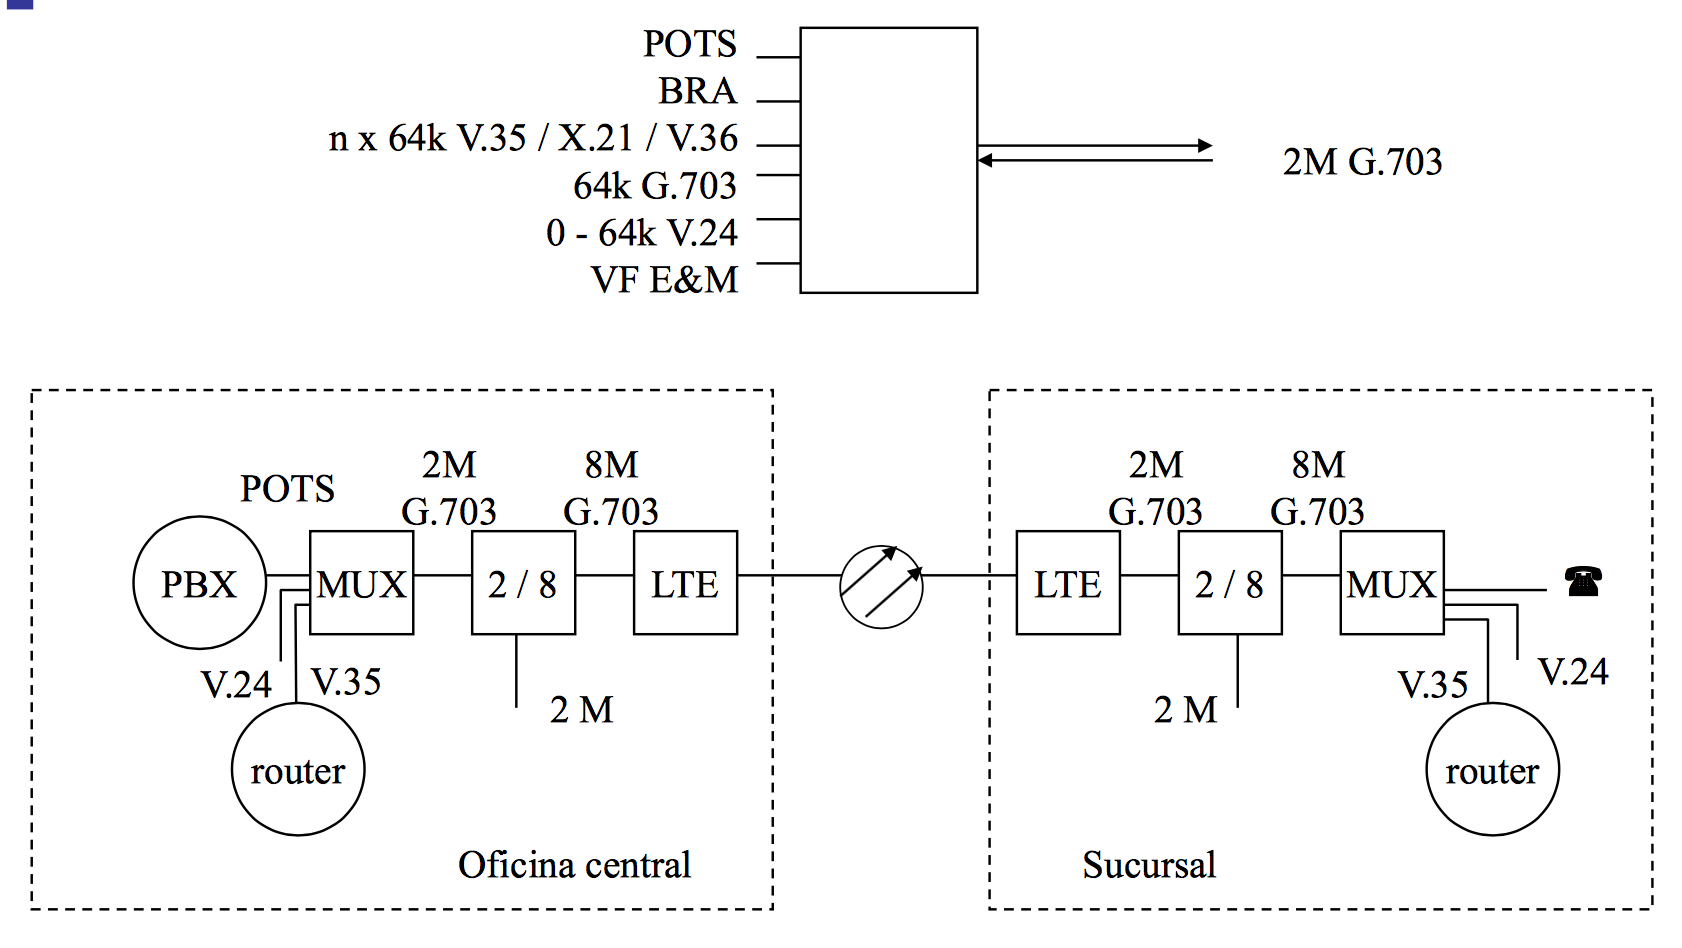
\includegraphics[scale=0.2]{images/MuxTerminal}
	\end{center}

\textbf{Multiplexores de Inserción y Extracción}

	\begin{center}
		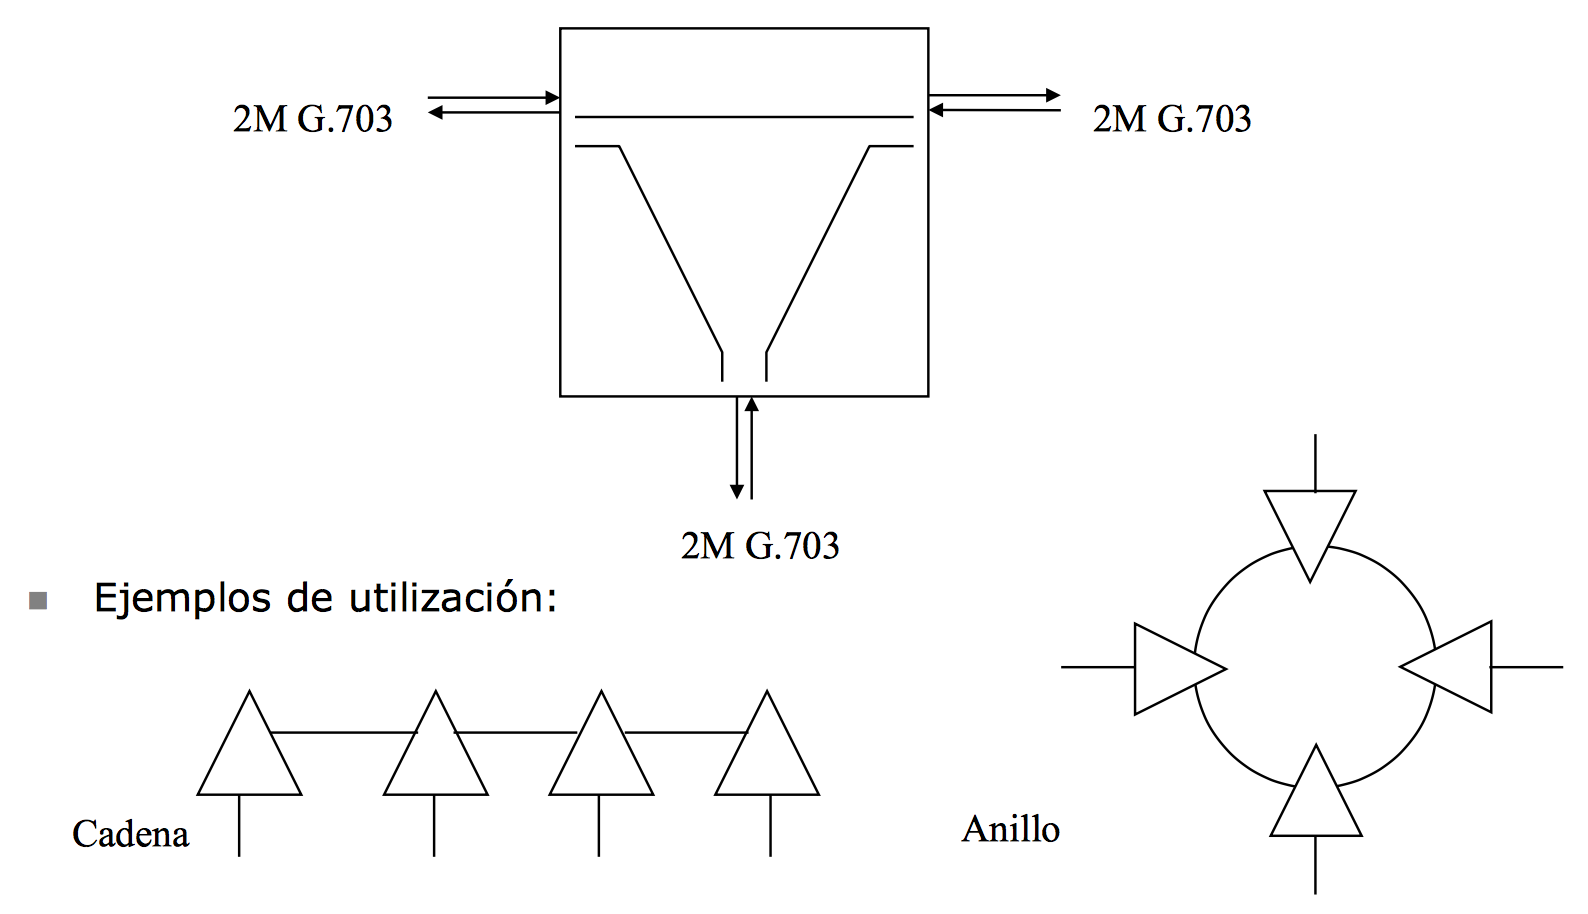
\includegraphics[scale=0.2]{images/MuxExtra}
	\end{center}

Tipos de conexiones:

	\begin{itemize}
	\item Punto a punto
		\begin{center}
			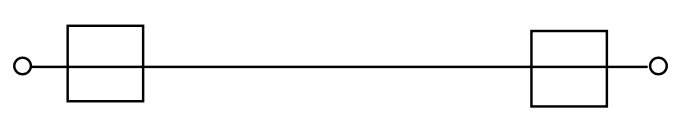
\includegraphics[scale=0.2]{images/P2P}
		\end{center}
	\item Punto a Multipunto
		\begin{center}
			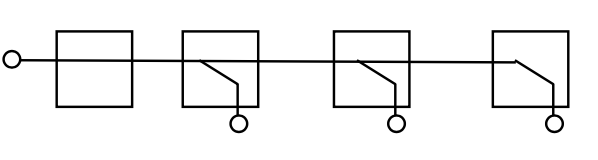
\includegraphics[scale=0.2]{images/P2M}
		\end{center}
	\item Punto a Multipunto
		\begin{center}
			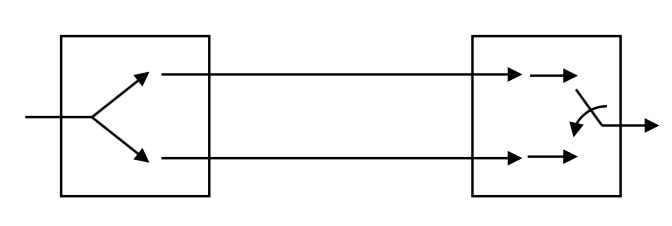
\includegraphics[scale=0.2]{images/Uni}
		\end{center}
	\item Protección de circuitos: sistemas propietarios
	\end{itemize}

\textbf{Cross connect}

	\begin{center}
			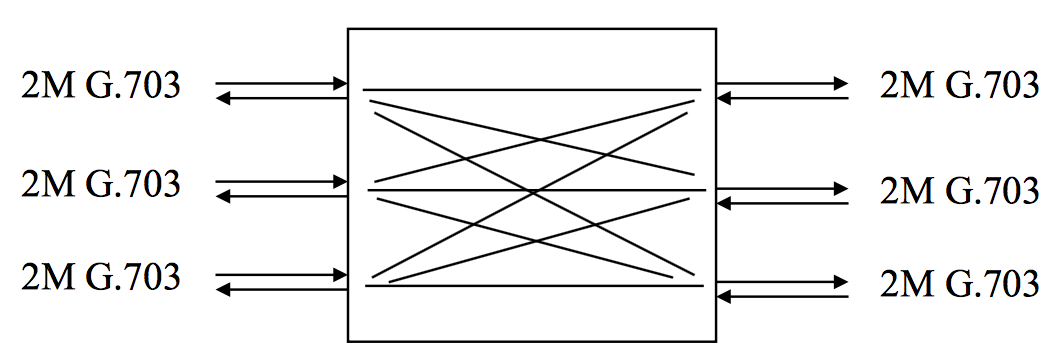
\includegraphics[scale=0.2]{images/Cross}
		\end{center}

\hrulefill

\subsection{SDH}

\subsubsection{Introducción}

\subsubsection{Velocidades SDH-SONET}

\subsubsection{Topologías de Red}

\subsubsection{Arquitectura SDH}

\subsubsection{Estructura STM-1/STM-N/STM-Nc}

\subsubsection{Tara de Sección}

\subsubsection{Contenedores y Punteros}

\subsubsection{Multiplexación y Mapeado de señales PDH sobre SDH}

\subsubsection{Gestión de red SDH}

\subsubsection{Protección en SDH}

\subsubsection{Sincronismo}

\subsubsection{Arquitectura de un operador}




































%\vfill

%\end{multicols}

\end{document}